%%%%%%%%%%%%%%%%%%%%%%%%%%%%
% Master's Thesis          %	    										
% Fabian Burth, 2022-08-01 %
%%%%%%%%%%%%%%%%%%%%%%%%%%%%	

\npchapter{System Design}
This chapter describes the technical design of the \textit{Security and Compliance Data Lake}. It covers the conception of the data model, the selection of a database, the design of the API and the complete application architecture. Thereby, it especially discusses alternatives and focuses on giving detailed information about the ideas and motives that led to specific design decisions.

\section{Requirements} \label{sec:Requirements}
Before actually going into the details of the systems design, the requirements have to be specified since they are at the core of every design decision.  

\subsection{Functional Requirements}
Table \ref{tab:Requirements} provides a condensed list of the functional requirements for the \emph{Security and Compliance Data Lake}. Thereby, every requirement is described by a short and precise but abstract statement of what functionality the system must have and an additional explanation which also includes an example. Moreover, there is a column categorizing the requirements as priority 1 or 2.\par 
\emph{Priority 1} is functionality deemed necessary for the \emph{Security and Compliance Data Lake} in order to solve the limitations and problems of the state of the art approach. Furthermore, priority 1 functionality is usually functionality that has to be considered in the design process and otherwise cannot be easily added without foundational remodeling.\par
\emph{Priority 2} functionality describes convenience features which are less urgent and may easily be added later on.
\begin{xltabular}{\linewidth}{|l|X|l|}
	\hline \hline \rowcolor{lightgray} \multicolumn{3}{ |l| } {\cellcolor{lightgray}{\textbf{Requirements}}}
	\\ \hline \rowcolor{lightgray}\textbf{Ref.\#} & \textbf{Functionality} & \textbf{Prio.}
	\\ \hline
	\endfirsthead
	
	\hline \hline \rowcolor{lightgray}\multicolumn{3}{|l|}{\cellcolor{lightgray}{\textbf{Requirements}}} \\ \hline \rowcolor{lightgray} \textbf{Ref.\#} & \textbf{Functionality} & \textbf{Prio.}\\ \hline
	\endhead
	
	\hline \multicolumn{3}{|r|}{{Continued on next page}} \\ \hline
	\endfoot
	
	\hline \caption[Requirements for the Security and Compliance Data Lake]{Application Requirements} \label{tab:Requirements}
	\endlastfoot
	
	R.1 & The SCDL shall be able to consume and store metadata from multiple different data sources.\newline\newline

	The SCDL shall be able to work with any kind of metadata about software components.	Therefore, it has to be able to handle the results of multiple different scanning tools as well as other kinds of data sources like build tools. As an example, it may have to consume data provided by \emph{Black Duck Binary Analysis (BDBA)}, Mend but also Jenkins. Thus, it has to be considered that besides vulnerabilities and licenses, a variety of other metadata types may need to be added in the future. & 1\\
	\hline
	R.2 & The SCDL shall store the metadata from different data sources without aggregation\footnotemark{}.\newline\newline
	Different tools that generally serve the same purpose may provide similar information. As an example, BDBA and Mend are both SCA tools and therefore provide overlapping results. To ensure that no data is lost, this information shall not be combined and aggregated before storing.
	\footnotetext{\textit{aggregation} in this context means to merge the data about a package of e.g. a BDBA scan and a Mend scan to a single package entity instance} & 1\\
	\hline
	R.3 & The SCDL shall provide the metadata from different data sources with aggregation\footnotemark[\value{footnote}].\newline\newline
	As mentioned before, to ensure no data is lost, the data from different data sources shall be stored without aggregation. Anyway, to be consumed by a user, this data shall be aggregated. As an example, when querying all packages contained in a specific resource, the result returned by the SCDL shall not contain the same package twice in different representations, if it was identified by BDBA and by Mend. Instead, the result shall contain an aggregated representation of the package. Thus, some kind of aggregation layer is needed which provides transparency regarding the data sources. & 1\\
	\hline
	R.4 & The SCDL shall provide a level of aggregation\footnotemark{} to group sources and resources.\newline\newline
	\footnotetext{\textit{aggregation} in this context refers to the ''whole/part'' semantic of the word \cite{UML}. Thus, since resources and sources are comprised of packages, they are both aggregations of packages. On a model level, the same applies for the relationships between packages and vulnerabilities or licenses as well as between entire deployments and the deployed resources.}
	As pointed out before, one problem also with SBOMs is the disconnection of the artifact metadata and the deployment information. To bridge this gap, an additional aggregation level for grouping artifacts is necessary. As an example, this additional aggregation level shall enable to group all resources contained in a specific product version. & 1\\
	\hline
	R.5 & The SCDL shall enable users to query the metadata on different levels of aggregation\footnotemark[\value{footnote}].\newline\newline
	As an example, a user shall be able to query for all vulnerabilities in a specific resource, thus, query on the aggregate level of resources. But a user shall also be able to query for all vulnerabilities in an entire specific deployment, thus, querying on the aggregate level of deployments (querying on this level of aggregation enables to answer where Log4j is deployed). & 1\\
	\hline
	R.6 & The SCDL shall enable users to perform assessments.\newline\newline
	The relevance of specific pieces of information such as vulnerabilities or licenses depends on the usage context. As an example, while the internal usage of an altered OSS with a copyleft license is lawful, the distribution is not. Therefore, a possibility has to be provided to assess such pieces of information in the context of their occurrence. & 2\\
	\hline
	R.7 & The SCDL shall provide common data aggregation and filter functions for the queries.\newline\newline
	As an example, a user shall be able to filter for the vulnerability with the highest CVSS within a resource or shall be able to get the count of vulnerabilities within a resource. & 2\\
	\hline
	R.8 & The SCDL shall enable users to query the metadata in the common SBOM formats.\newline\newline
	In order to be able to fulfill the governmental requirements of the executive order mentioned in \ref{sec:SBOM} ''Software Bill of Materials'', the SCDL has to provide a way to query the metadata in the common SBOM formats. As an example, a user shall be able to query the SPDX document for a specific resource. & 2\\
\end{xltabular}

So, by fulfilling this functional requirements, the \emph{Security and Compliance Data Lake} may actually serve as a central application for storing and querying software metadata. Thereby, solving the problem of metadata being distributed throughout the development life cycle and bridging the gap between artifact metadata and deployment information.

\subsection{Non-functional Requirements} \label{sec:Non-functional Requirements}
Since this shall be a prototypical implementation, there is a strong focus on fulfilling the functional requirements. Thus, no concrete limits regarding performance or scalability such as a maximum response time of 5 seconds or support for up to 1000 concurrent users are set here. Considering the novelty of the topic, there is very few reference data and therefore, such specifications would be premature. However, for a central metadata store which may prospectively power dashboard web applications for monitoring purposes, scalability and performance definitely have to be considered in design decisions already.

\section{Data Model} \label{sec:Data Model}
Before discussing the actual data model, a brief revision of the relevant terms and entities.\par Artifact is an umbrella term for sources and resources. The definition of sources and resources is the same as introduced by the OCM.\par 
Resources describe delivery artifacts, intended for deployment into a runtime environment (e.g. executeables or OCI Images) or additional content relevant for deployment mechanisms (e.g. helm charts).\par
Sources describe the artifacts that are used to generate the delivery relevant artifacts (e.g. source code).\par
Compliance scanners usually scan entire source code repositories or binaries. Through different methodologies, these tools detect the packages contained in these scanned artifacts on a best effort basis. In the context of this work, packages are defined as functional units composing artifacts, whereby it is usually a collection of files forming a library which is imported in the source code.\par
By subsequently matching these packages against different databases such as the NVD, introduced in section \ref{sec:Vulnerability Management} ''Vulnerability Management'', known vulnerabilities and licenses are identified. To give a better idea of these results, figure \ref{fig:bdbaResult} in the appendix shows a snippet returned from the API of BDBA. The results on their own are useful already and provide interesting data about the above mentioned entities. But it is still loose metadata that lacks context information such as which product versions contain the corresponding entities.\par
Therefore, an additional entity type to conduct further aggregation is required. The OCM already introduced such an entity type, the component.\\

To conclude this, from a high level perspective, the important entities are \emph{components}, \emph{sources}, \emph{resources}, \emph{packages} and the information attached to these entities such as vulnerabilities and licenses. To generalize this and abstract away from specific data sources, the entities representing these types of metadata are called \emph{info snippets}.\par
So these entities are the starting point for the data model. From here on, it is getting rather complex and abstract. To still keep the explanations tangible, figure \ref{fig:DataModel} shows an \emph{entity-relationship model (ERM)} describing the data model. This may be used as a reference point throughout the following paragraphs, discussing the design decisions leading up to the specific entity types, relationships and cardinalities.

\begin{figure}[H]
	\centering
	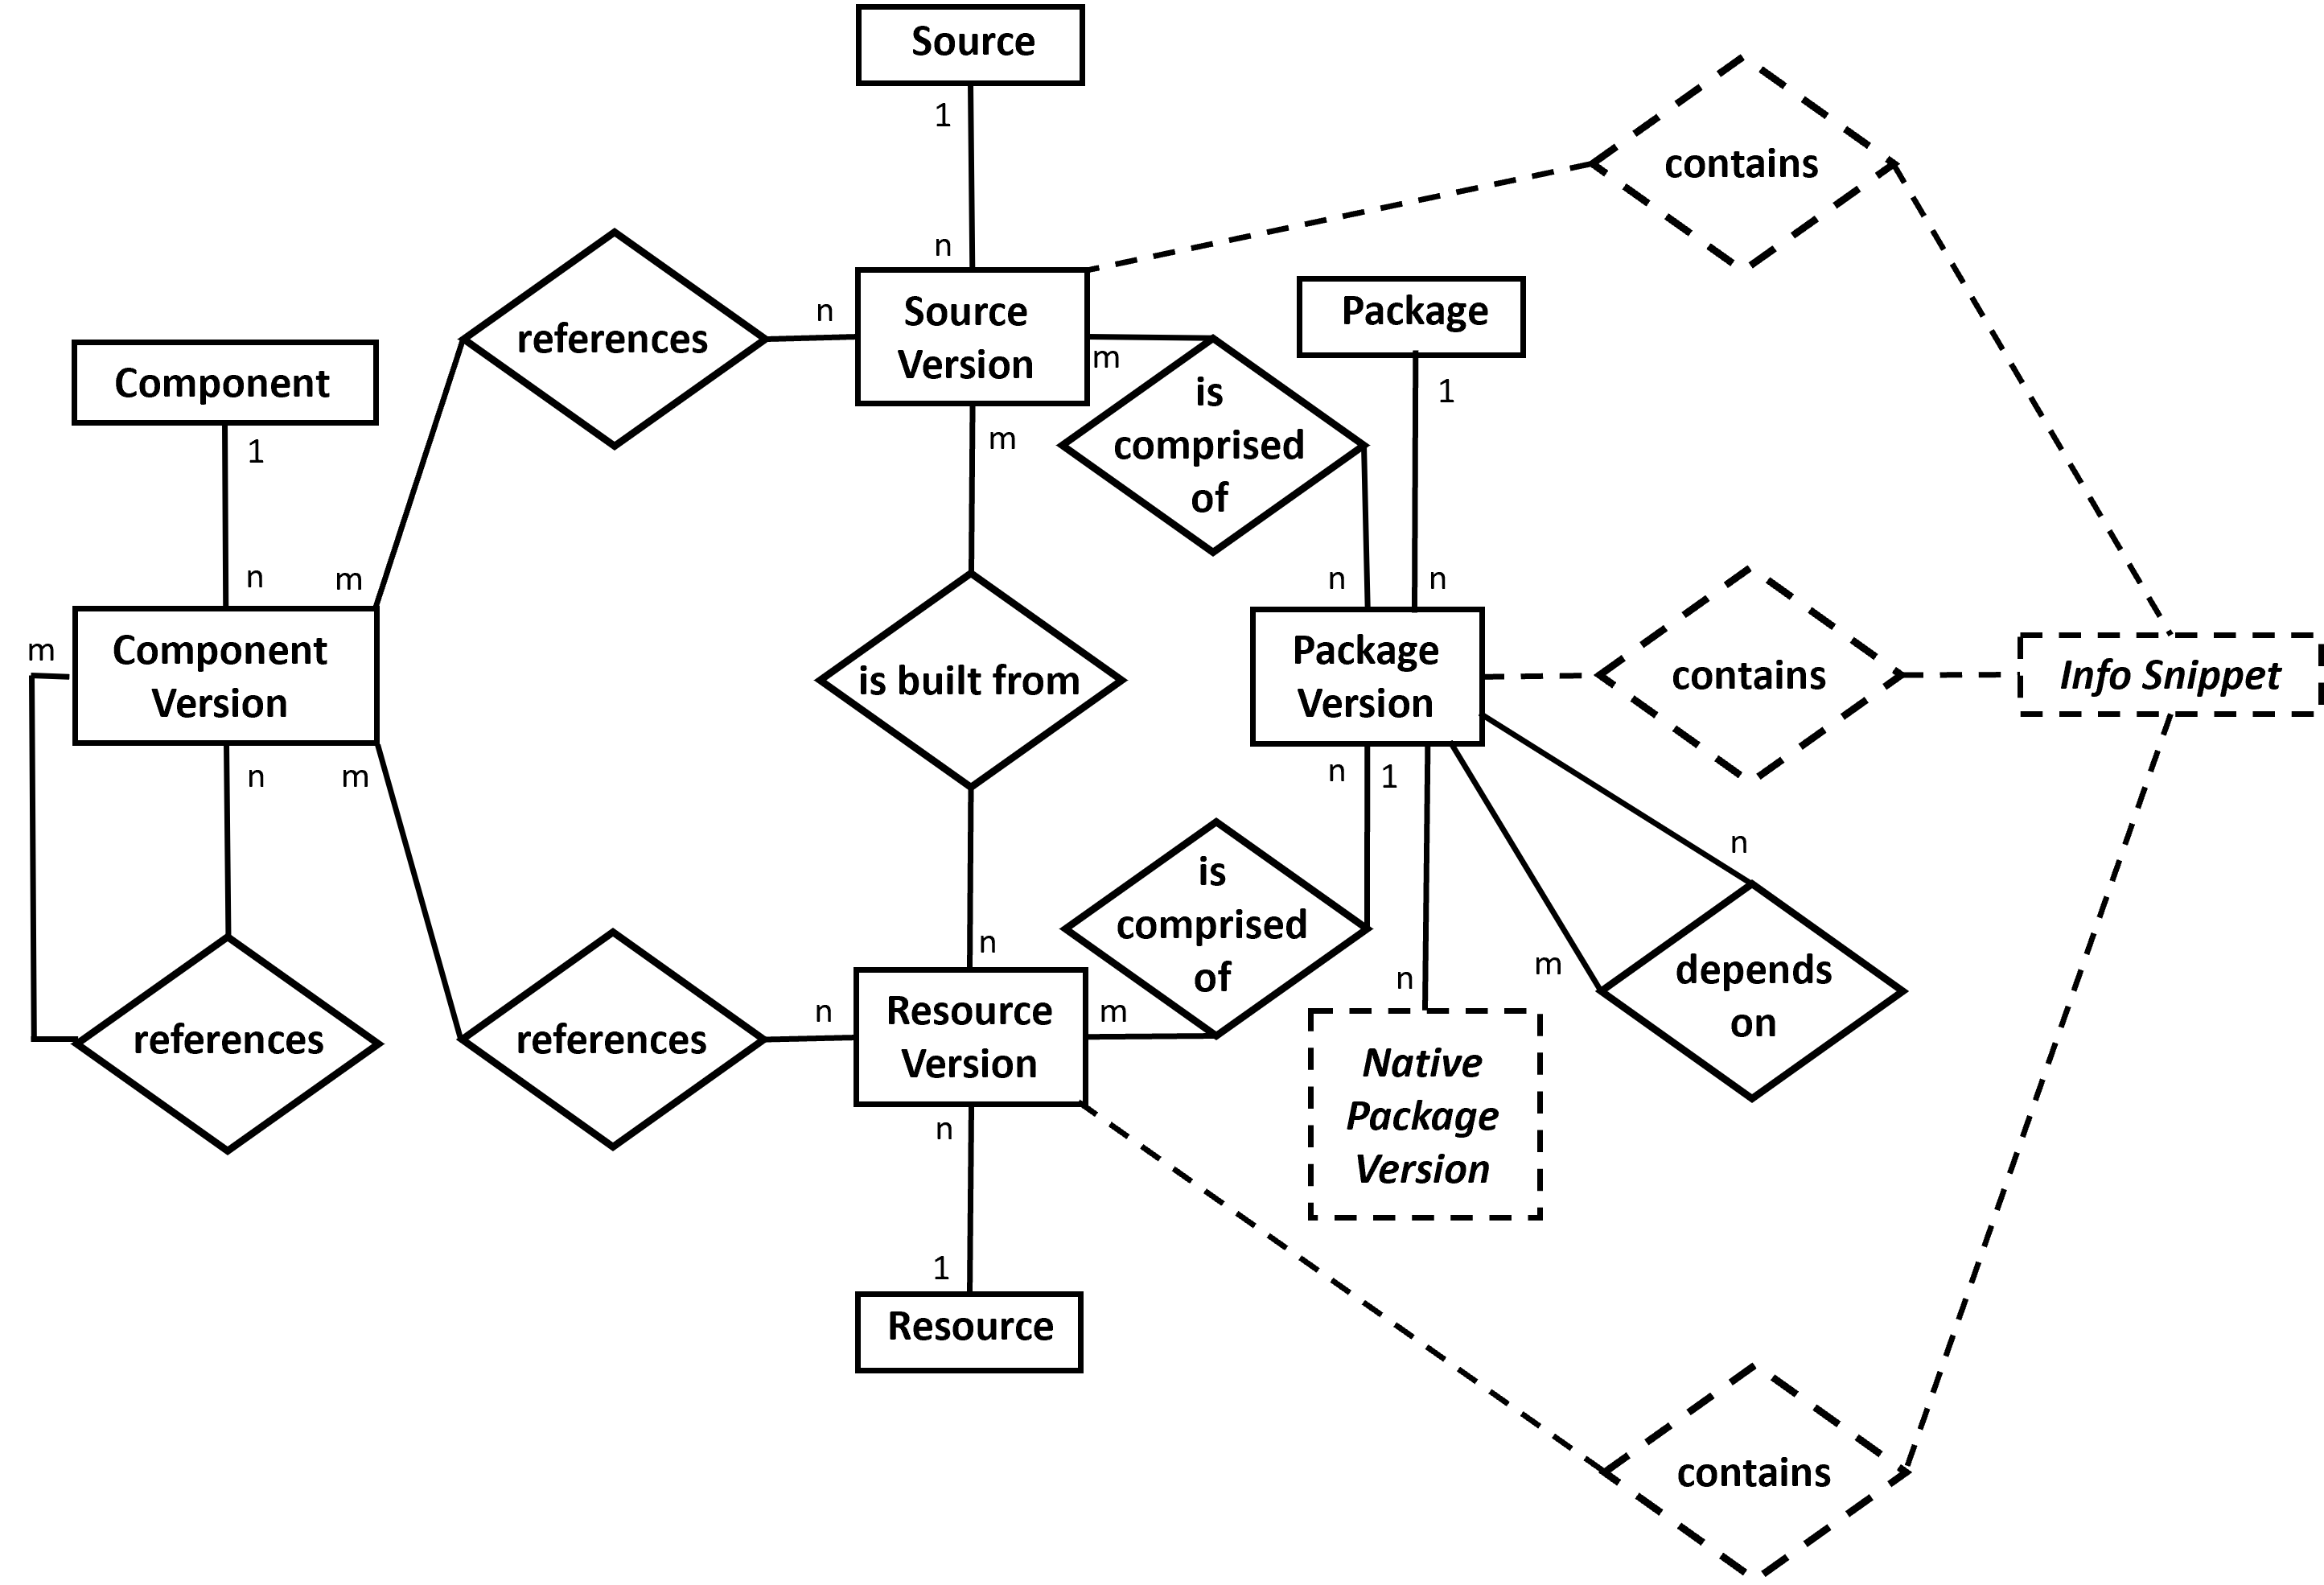
\includegraphics[scale=0.65]{datamodel}
	\caption[Meta Data Model]{Meta Data Model \source{Own Representation}}
	\label{fig:DataModel}
\end{figure} 

Even though the motivation behind every element may not be obvious immediately, the model as a whole should feel quite familiar from the abstract data lake design.\par
The previous chapter shows that the \emph{Data Lake} is built around and based on the OCM. Consequently, the data model is also inspired by the OCM. As mentioned above, especially the entity type \emph{component} is lend from its model elements. Since this thesis is written within SAP Gardener, a seamless integration of the \emph{Security and Compliance Data Lake} such as described in the previous chapter is, of course, also a requirement, even though it is not explicitly listed.\par
But to stress this again, the \emph{Security and Compliance Data Lake} is nonetheless designed independent of the OCM. Thus, as described in the previous chapter, it is entirely possible to use a different kind of \emph{Component Model}.\par 
As an example, if one is able to provide the capabilities of a \emph{Component Model} and express the concept of \emph{components} and \emph{artifacts} with the means of the SPDX standard, one could use SPDX instead of OCM to provide this structural information. Or, since SPDX is not optimal for this purpose, one could create and use an own \emph{Component Model}.\par
An additional notion, there is generally no necessity to distinct between \emph{sources} and \emph{resources}. \emph{Sources} could be treated as \emph{resources}, at the only cost of losing the connecting ''is built from''-information between the two entity types.

\subsection{Meta Data Model}
Contrary to common ERMs, the one in figure \ref{fig:DataModel} does not have any properties. There are two major reasons for this. Firstly, the just mentioned independence of a specific component model would hardly be possible if the data model would define fixed predefined properties for each entity type. Secondly, the different scanning tools provide a wide range of information about packages, and other data sources apart from scanning tools may also be added. It is therefore practically impossible to foresee what properties may be needed. Besides, these may vary depending on the user of the \emph{Security and Compliance Data Lake}.\par
Another special feature of above ERM are the entity types and relationships illustrated with dashed lines. These represent \emph{classes of entity types} and their potential relationships. Since the whole set of data sources cannot be known upfront, the whole set of potentially required \emph{Info Snippets} cannot as well. As already mentioned in several examples before, when adding a build tool as data source, an entity type \emph{Build Information} may be needed. Also, the relationships of different \emph{Info Snippet} entity types may vary. While a \emph{Vulnerability} or a \emph{License} is usually \emph{contained} in multiple \emph{Package Versions} leading to a (n:m)-relationship, a \emph{Build Information} is usually associated to one \emph{Resource Version} leading to a (1:n)-relationship. But generally, \emph{Info Snippets} could be associated to any other entity type in the data model with any cardinality.\par
\emph{So, the data model allows to configure arbitrary properties for each entity type. Moreover, it allows to instantiate multiple entire entity types of these classes of entity types, also with arbitrarily configurable properties. Therefore, it is actually a meta data model.}\\

This kind of flexibility is necessary to enable R.1 (consume and store metadata from multiple different data sources).\par 
The \emph{Native Package Version} correspondingly illustrates the representation of a package, native to a concrete data source. Thus, entity type instances of \emph{Native Package Versions} may be \emph{BDBA Package}, \emph{Mend Package} or even \emph{Jenkins Package}. So if all three data sources provide information about the exact same \emph{Package Version}, each representation may be stored without a need to merge their properties before storing. Thereby, this enables R.2 (store metadata from different data sources without aggregation).\par 
Then, a set of properties commonly provided by all of the data sources may be aggregated on \emph{Package Version} level, thereby also enabling R.5 (provide the metadata from different data sources with aggregation). So, all these \emph{Native Package Versions} representing the exact same package are related to the same \emph{Package Version} on the model level. As the different data sources may use different identifiers for the packages, the merging process cannot be triggered automatically. Hence, until a human defines that the \emph{BDBA Package}, the \emph{Mend Package} and potentially also the \emph{Jenkins Package} are actually representations of the same package, no merging is done and each is related to a different \emph{Package Version}.\par
The previous chapter frequently mentioned the need for a technology-agnostic uniform identification scheme. The aggregation of \emph{Native Package Versions} through \emph{Package Versions} allows to configure such a technology-agnostic uniform identification scheme for packages within the context of the \emph{Data Lake} (thereby, the uniform identification scheme may just be a simple ID or UUID).\\

\noindent So, after explaining the special features of above ERM, the general model may be discussed.\\

\noindent\textbf{Component, Component Version and Relationships}\\
The basic entity type \emph{component} is broken down into two distinct entity types, \emph{Component} and \emph{Component Version}. As immediately noticeable, this distinction is done for each of the basic entity types. \emph{Component} is a purely abstract entity type. It merely groups all the versions of the same component together. Thereby, the \emph{Component} may provide information about the semantics of this grouping such as whether this \emph{Component} describes a specific software product or whether it describes all software products used by a department. Thus, information that is identical for all versions of this component and would have to be stored redundantly for each \emph{Component Version} otherwise. Naturally, there are multiple \emph{Component Versions} of each \emph{Component}. Therefore, the (1:n)-cardinality here is self-explaining.\par 
As established by the previously described grouping semantic of \emph{components}, a \emph{Component Version} may reference multiple other \emph{Component Versions}. For example, a \emph{Component Version} describing a specific version of a software product may reference multiple other \emph{Component Versions} such as \emph{Component Versions} describing specific versions of a web server, a service and a database. Reciprocal, a \emph{Component Version} may of course be referenced by multiple \emph{Component Versions}. For example, a \emph{Component Version} describing a web server may be referenced by several \emph{Component Versions} describing different versions of the same software product or entirely different software products. Thus, this is a recursive (n:m)-relationship. There may also be a need to store additional occurrence specific metadata as properties of the \emph{references}. Considering the above example, such occurrence specific metadata may provide information about the usage of the web server within the deployment, hence whether it is used as a HTTP server or as a load balancer. Together, these model elements fulfill requirement R.4 (provide an aggregation level to group sources and resources).\par
Furthermore, a \emph{Component Version} may also reference multiple \emph{Source Versions} and \emph{Resource Versions}. As an example, the \emph{Resource Versions} composing the web server and the \emph{Source Versions} from which the respective \emph{Resource Versions} were built. As before, with the recursive relationship of \emph{Component Versions}, the \emph{Source Versions} and \emph{Resource Versions} may of course also be referenced by multiple \emph{Component Versions}, resulting in a (n:m)-relationship. Again, there may be a need to store additional occurrence specific metadata as properties of the \emph{references}. Specifically, these \emph{references} may be used to store \emph{triage} information. As this \emph{reference} describes the usage context of the \emph{Artifact}, one may for example decide whether a copyleft license is or is not acceptable here.\\ 

\noindent\textbf{Artifact, Artifact Versions and Relationships}\\
The relationship between \emph{Source} and \emph{Source Version} as well as between \emph{Resource} and \emph{Resource Version} is similar to the relationship between \emph{Component} and \emph{Component Versions}. But the abstract \emph{Source} and \emph{Resource} entity types actually do have a concrete purpose apart from preventing redundant storage of certain properties. In this case, these abstract entities may have properties to store \emph{triage policies}. As an example, one may store that a specific vulnerability may be ignored for the usage of \emph{Resource Versions} v1.0.0 to v1.2.3 of a respective \emph{Resource} within \emph{Component Versions} v1.4.2 to v1.4.12 of a specific \emph{Component}. The \emph{references} and the abstract \emph{Source} and \emph{Resource} entity types thereby enable the fulfillment of requirement R.6 (enable users to perform assessments).\par 
\emph{Resource Versions} may also reference the \emph{Source Versions} they are built from. A \emph{Resource Version} may be built from multiple \emph{Source Versions} and a \emph{Source Version} may be used to build multiple \emph{Resource Versions}. This also results in a (n:m)-relationship.\par
Since \emph{Artifacts} are comprised of \emph{Package Versions} and the same \emph{Package Version} may occur in multiple \emph{Artifacts}, both \emph{Source Version} as well as \emph{Resource Version} have a (n:m)-relationship to \emph{Package Version}. Again, there may be a need to store additional occurrence specific metadata as properties of the \emph{is comprised of} relationship.\\

\noindent\textbf{Package, Package Version, Native Package Version and Relationships}\\
The relationship between \emph{Package} and \emph{Package Version} is again similar to the relationship between \emph{Component} and \emph{Component Versions}. But as already explained, \emph{packages} are broken down even further into three different entity types and thereby three aggregate levels. Since several data sources may provide different representations, thus different \emph{Native Package Versions}, of the same \emph{Package Version}, the cardinality of this relationship is (1:n). \emph{Package Versions} frequently \emph{depend on} other \emph{Package Versions} and so on. This may lead to quite long chains of dependencies. This has to be kept in mind as these transitive dependencies are also relevant when trying to answer the question, whether a certain \emph{Artifact} or \emph{Component} contains a specific \emph{Package} such as Log4j, and its corresponding vulnerabilities.\\

\noindent\textbf{Info Snippet and Relationships}\\
Finally there is the \emph{Info Snippet} class of entity types. As explained above, different \emph{Info Snippet} entity types may have relationships to different entity types with different cardinalities.

\subsection{Insights into the Development Process} \label{sec:Insights into the Development Process}
At this point, some insight into the development process may be beneficial to understand the design decisions. The scope of this central data store was initially much narrower. The first PoC was actually strictly bound to the OCM. Therefore, the data model predefined the properties of \emph{component} and \emph{artifact} entity types. As it was bound to the OCM, there was no issue in doing so.\par
But the data model also predefined the properties of the \emph{package} entity types. In fact, the third aggregate level for \emph{packages}, \emph{Native Package Version}, did not exist at all. Instead, the \emph{Package Version} entity type had a set of properties that was hoped to be common and harmonizable throughout all prospective data sources. At this time, the application was also tailored to only having scanning tools as data sources. Therefore, to define this set of properties, the API documentations of different scanning tools were analyzed for the common and most important properties, especially the ones of BDBA and Mend \cite{MendAPI}. Additionally, to get a better understanding, both scanners were used on some artifacts to get sample data. Then, the provided attributes were narrowed down and some interviews with developers were conducted. A huge effort was made here, as this was such an important decision. Also, instead of having the \emph{Info Snippet} class of entity types, there was only a \emph{Vulnerability} and a \emph{License} entity type whose sets of properties were defined in the same process. Apart from the fact that there was already a substantial amount of disagreement between different developers which properties were actually required, by the time the PoC was finished, several new use cases were discovered that required additional properties and even entire additional entity types to provide other metadata than vulnerabilities or licenses.\par
This led to a change in perspective, interpreting the task of defining the right entity types with the right properties rather as a task to make the entire application extensible regarding the respective entity types and properties. But this flexibility and extensibility comes at the cost of a highly increased overall complexity. Apart from remodeling the data model, it also required a completely new architecture and completely different implementation. Thus, only after that, the scope widened drastically, also allowing other component models. Consequently, as a kind of disclaimer, the design process presented here is not exactly as chronological as it may initially seem, since it hides a complete development iteration leading up to the final concepts.

\subsection{Application of the Data Model} \label{sec:Application of the Data Model}
Although a great effort was made to make the data model as tangible as possible, it may still be hard to grasp due to its abstract nature, omitting properties and introducing classes of entity types. Therefore, this section discusses how this data model could be applied. As reference component model, the OCM is used and as reference data sources, only BDBA is used. This thereby also reveals a problem that has to be faced when applying this data model to a real world use case. The figure \ref{fig:RefDataModel} shows the corresponding data model instance.\par

\begin{figure}[H]
	\centering
	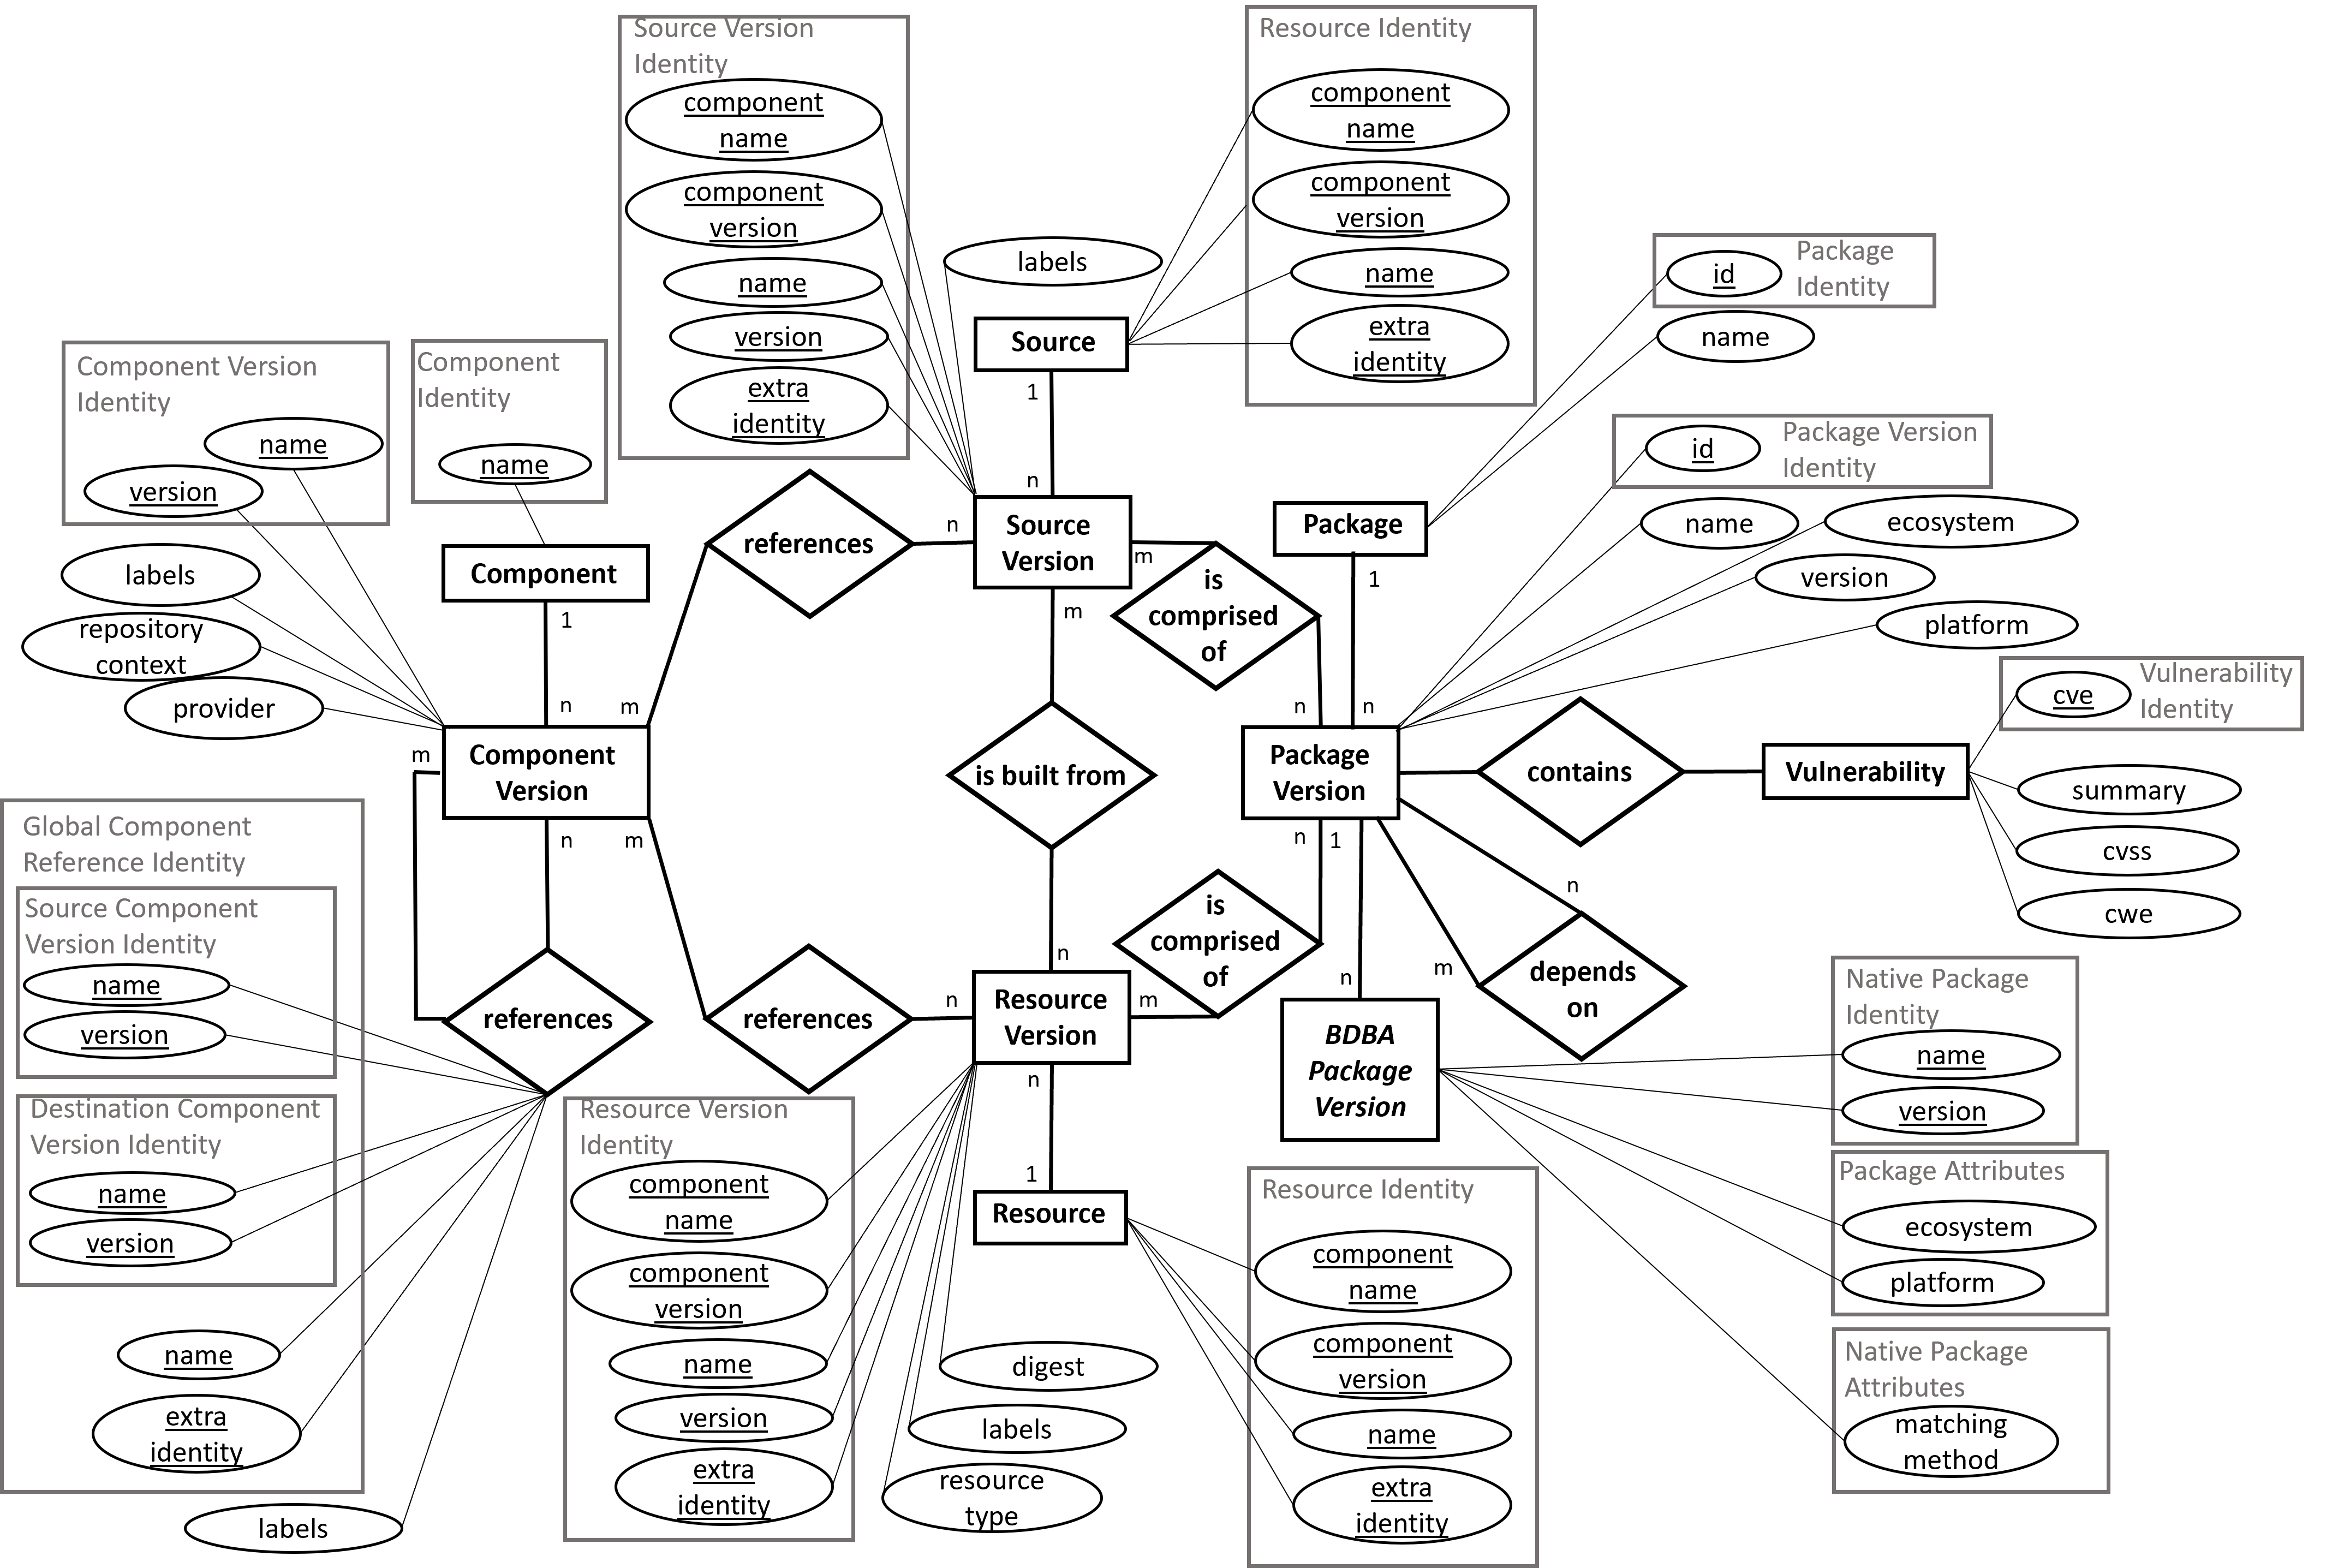
\includegraphics[scale=0.45]{refdatamodel}
	\caption[Data Model Instance]{Example Data Model Instance \source{Own Representation}}
	\label{fig:RefDataModel}
\end{figure}

The figure is very crowded. But this is necessary as the purpose of it is to provide a concrete and thorough illustration of how the meta data model may be applied to specific component models and data sources. Thus, it shows a concrete example of how to instantiate the model's entity types for a concrete environment with appropriate attributes.\par
The important aspect to point out here is the relationship between \emph{Component Version} and \emph{Source Version} and between \emph{Component Version} and \emph{Resource Version}. Although depicted as a relationship with (n:m)-cardinatility in compliance with the meta data model, due to the \emph{Component Version-Local Identity} of \emph{Source Version} and \emph{Resource Version}, these can actually only be (1:n)-relationships. There were detailed explanations about this in section \ref{sec:Open Component Model} ''Open Component Model''. The SAP Gardener team chose this initially rather non-intuitive specification of \emph{Source Versions} and \emph{Resource Versions} with \emph{Local Identities} since in practice, it is difficult to reliably determine whether two referenced technical artifacts are actually the same technical artifact.\par 
The following section further explain the issue and discusses different approaches of dealing with this \emph{artifact identity problem}. It thereby points out the use cases and limitations of each approach.\par
As the common software developer immediately attempts to translate this data model into tables, a corresponding exemplary relational model is shown in the appendix \ref{apx:Relational Model of the Example Data Model Instance}.  

\subsubsection{Artifact Identity Problem} 
\noindent\textbf{Artificial Identifiers}\\
The initial and most obvious approach is to treat technical artifacts just as components. Thus, assign a globally unique name and a version to each technical artifact. But the reason this works for components is that these are purely abstract or logical entities. Thus, there is no digital or rather technical twin such as source code or a binary that corresponds to a specific component. If there is, who guarantees that two \emph{Resource Versions} with the same name and the same version actually point to the same binary? Or reciprocal, that two \emph{Resource Versions} pointing to the same binary actually have the same name and version? Where and how would one look up this globally unique name of a \emph{Resource Version} in the first place?\par
A common approach in this situations are \emph{Uniform Resource Identifiers (URI)}. As introduced in section \ref{sec:Software Identification} ''Software Identification'', by providing a specification of how this URI is composed, standards such as \emph{purl} provide a way to create theoretically reproducible identifiers. Theoretically, because in practice composing this URIs still has to be done by people. Consequently, there is always room for interpretation and human error. Imagine a \emph{Resource Version} in two different \emph{Component Versions} referencing artifacts in two different repositories, for example \lstinline|github.com/example/nginx| with tag \lstinline|1.0.3| and \lstinline|github.com/example/nginx-webserver| also with tag \lstinline|1.0.3|. At this point, it is difficult to determine, whether these are technically the same artifact and should consequently have the same URI. Thus, this approach is unreliable and impractical.\\

\noindent\textbf{Origin URLs as Global Identifiers}\\
In order to guarantee that two \emph{Resource Versions} with the same URI actually point to the same binary and that two \emph{Resource Versions} pointing to the same binary actually have the same URI, this URI has to be a URL, pointing to the stored binary. Therefore, a coupling of identity and location is necessary.\par 
The straight forward approach to do this in practice is to use the URLs provided by the repositories. But, as the example above shows, this approach is not really flexible, as the identifiers have to be immutable even if the artifacts location changes.\par 
Therefore, in OCM the access attribute may be changed. Still in SAP Gardener technical artifacts and component descriptors are all replicated from a central development landscape into other landscapes. Only the access attributes' values change in this transport process. So the development landscape may serve as single source of truth, a \emph{central origin} for all artifacts, and the respective \emph{origin artifact URLs} of the access property in the development landscape could be used as \emph{global identifiers}. Even though the URLs in the access attribute of the component descriptors in other landscapes may differ from the global identifier of the artifact, as this \emph{identifier is the URL} used to copy the artifact to the location referenced by the URL in the new access attribute, it is the same per construction. So this approach is generally reliable and practical.\par
SAP Gardener did not consider this approach anyway, as it is more complex and globally unique identifiers for artifacts were not relevant for the original scope of the OCM, which was deployment automation.\\

\noindent\textbf{Digests as Global Identifiers}\\
Another option to determine whether two artifacts are technically the same, even though they are located in different repositories is to calculate a suitable \emph{normalized digest}.\par 
A \emph{digest} refers to a short, fixed-length string calculated through a hash function \cite{Cryptography}. There are several features in which artifacts may vary but that are irrelevant for their comparison. For example, the exact same source code file may provide different digests when hashed with the exact same hash method, depending on whether it is hashed on a windows or a linux machine. This is due to the different line endings, thus ''Carriage Return and Line Feed'' on windows and ''Line Feed'' on linux. In order to calculate a normalized digest, the input data for the hash function is prepared so that such irrelevant features do not have an impact on the digest. So, the input data is normalized.\par
This approach is generally reliable and clean, but there are again several problems. When looking at figure \ref{fig:RefDataModel} above, there is already a digest property available for \emph{Resource Versions}. As described in section \ref{sec:Open Component Model} ''Open Component Model'', this digest property specifies a hash function, a normalization function and the corresponding digest value. Although the primary reason for this is that different kinds of resources, for example executeables and OCI Images, may need different kinds of normalization functions, this also means that the same artifact may have different digest values in different \emph{Component Versions}.\par
Consequently, the digests need to be calculated in a standardized way, independent of the OCM. But even then, there is still another issue regarding the data model. There is no way to decide whether artifacts with different normalized digests may be different versions of the same artifact. Thus, the additional aggregate level, \emph{Source} and \emph{Resource}, required for triage policies is practically impossible to maintain.\\

\noindent\textbf{Component Local Identifiers}\\
This is the approach used in the OCM. This concept was explained in detail in section \ref{sec:Open Component Model} ''Open Component Model''. Although it is not intuitive, only having \emph{local identifiers for artifacts is still functional regarding the goals which shall be achieved by the data model}.

\begin{figure}[H]
	\centering
	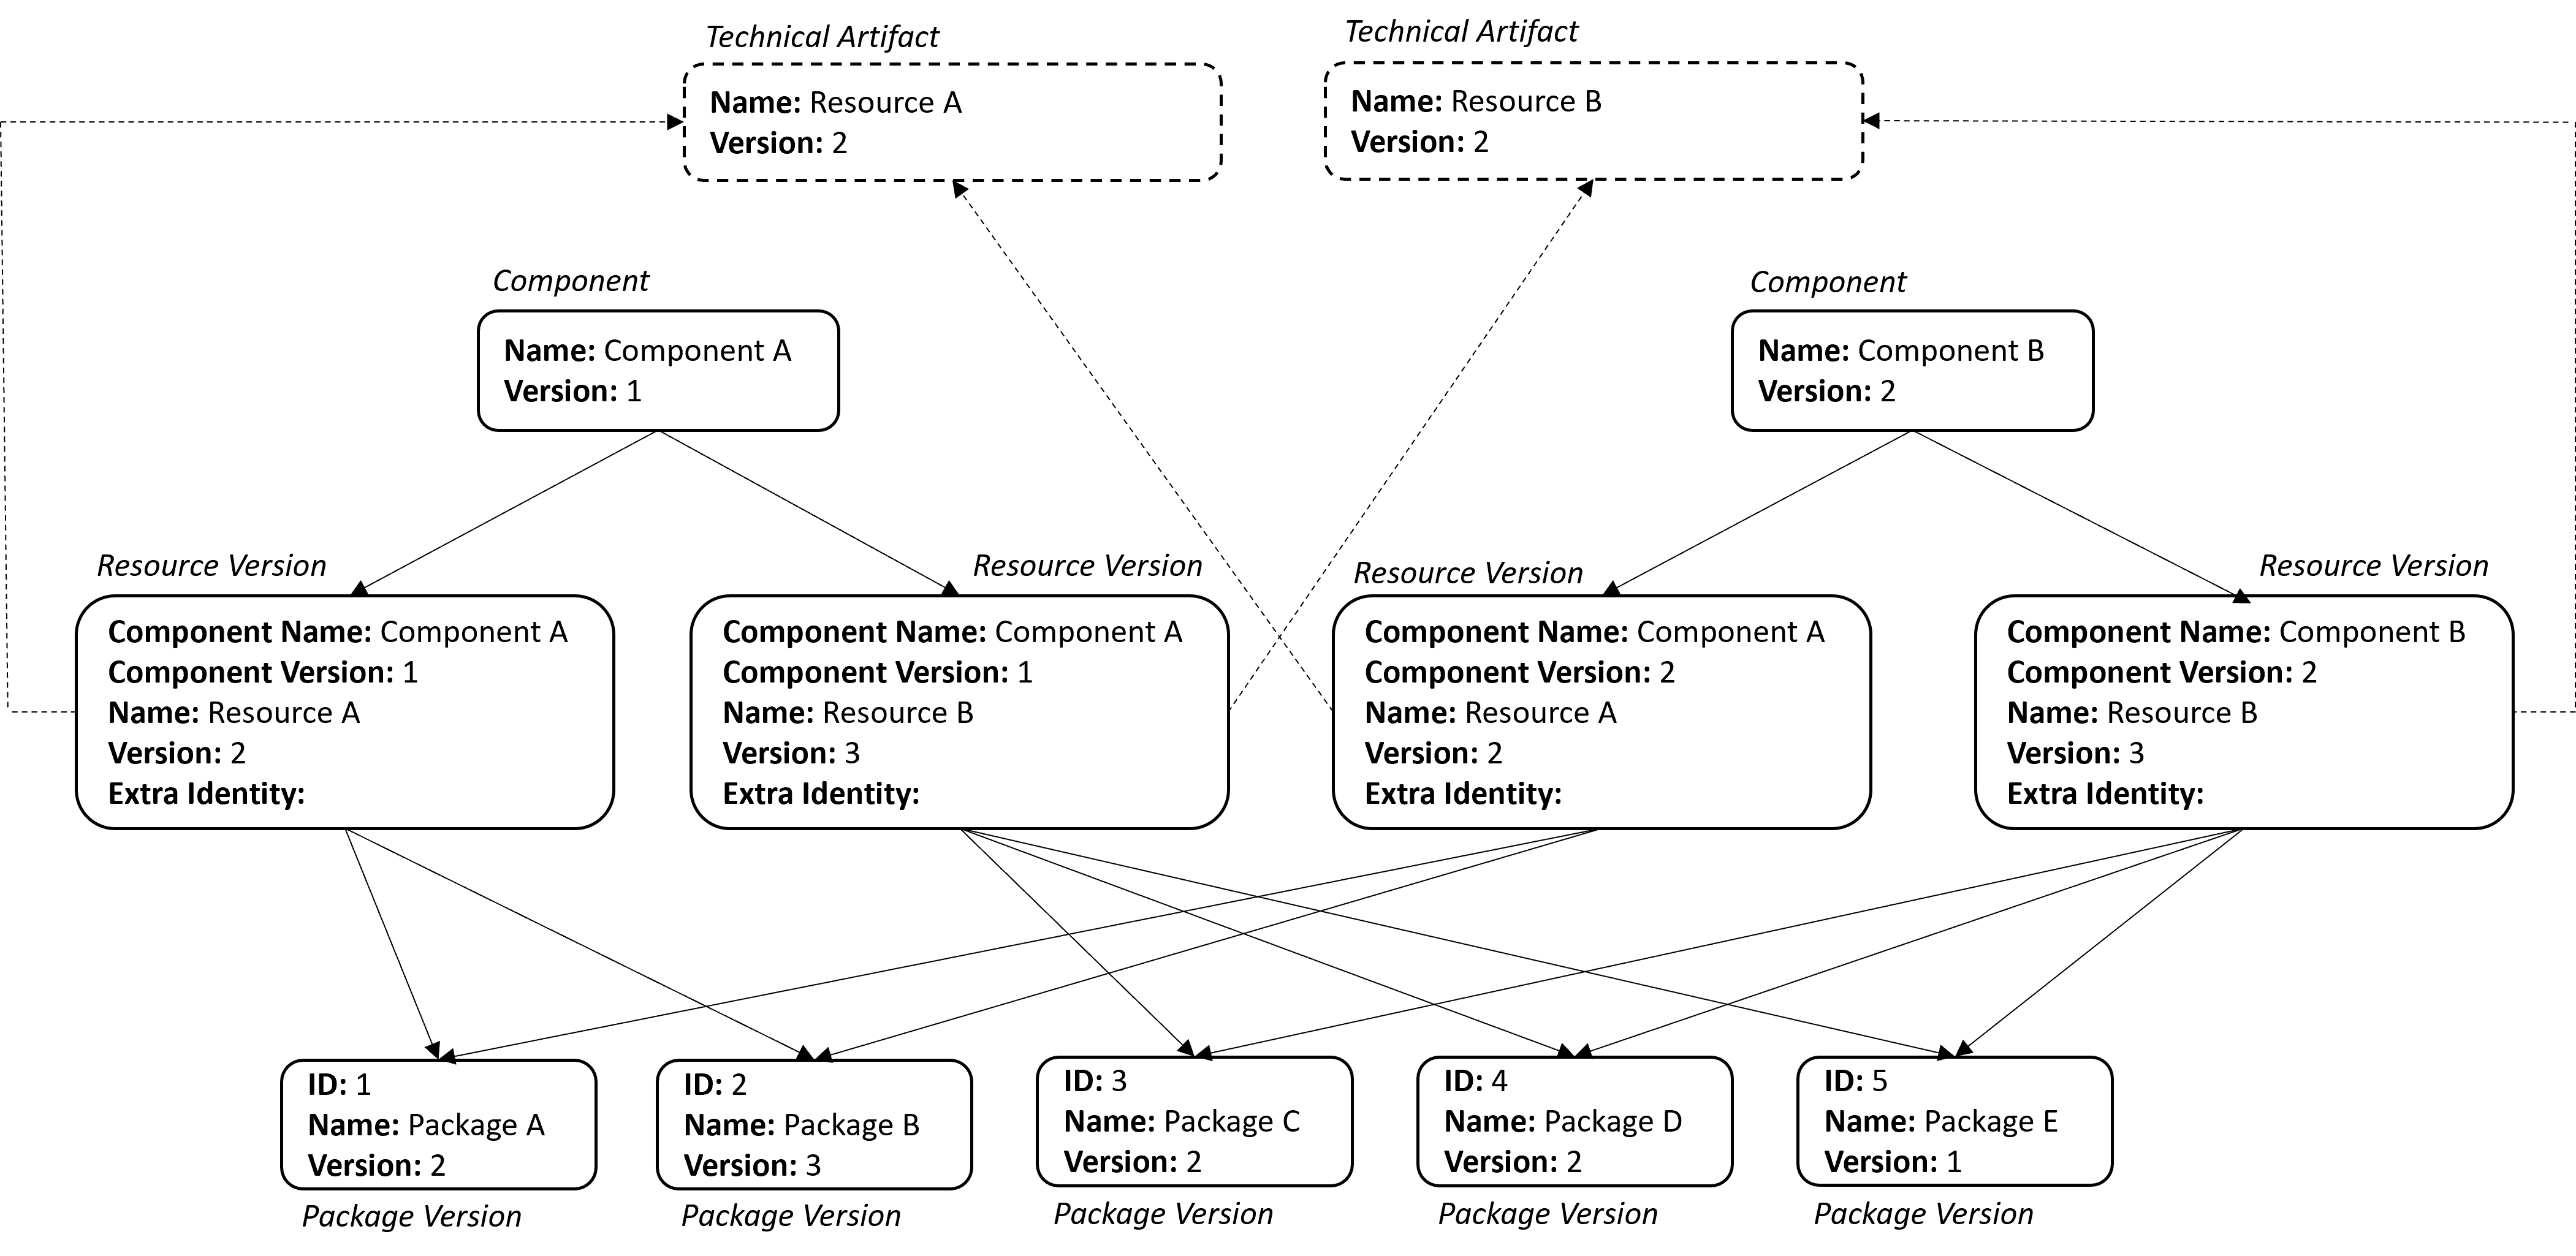
\includegraphics[scale=0.45]{localartifactidentity}
	\caption[Local Artifact Identities]{Local Artifact Identities \source{Own Representation}}
	\label{fig:LocalArtifactIdentity}
\end{figure}

Figure \ref{fig:LocalArtifactIdentity} shows two components that reference the exact same technical artifacts. But since the \emph{Identity} of \emph{Resource Versions} is local, the component name and version are part of the \emph{Resource Versions' Identity}, as also shown in figure \ref{fig:RefDataModel}. Thus, it appears as they are referencing different artifacts. But as the packages comprising the \emph{Resource Versions} are identified by scanning the technical artifact accessed through the access property, they are the same for the \emph{Resource Versions} which practically reference the same technical artifact.\par 
So, for answering questions such as: ''Which deployment contains Log4j and its corresponding vulnerabilities?'', the local artifact identities do not make a difference.\par 
In practice, it may also be assumed that within a \emph{Component}, \emph{Resource Versions} with the same name but different version numbers are in fact pointing to different versions of the same technical artifact. \emph{Thus, local identities are usually kept stable among successive version of a Component}.\par 
Therefore, the \emph{Resource} aggregate level is also possible. But its scope and the scope of \emph{triage policies} within these entities respectively is of course limited to a certain \emph{Component}.

\section{Database}
After the application context and data model are defined, a suitable database has to be selected. Therefore, this section analyzes the most relevant database technologies regarding their applicability as a central data store based on the previously defined data model.

\subsection{Requirements for the Database}
The most important aspect regarding the suitability of a database technology is the purpose of the data store and the respective kind of usage. Several relevant factors depend on this information. Is read or write performance more important? What may be acceptable delays when reading or writing data? What kind of queries may be used most frequently? Will the data be used for statistical analysis and require a lot of aggregation over dimensions such as time periods or locations? Are the entities highly inter-connected and require traversing relationships efficiently? How many users may need to access the data concurrently? May the database need to be distributed?\\\\
\textbf{Write Performance:} The data may be provided by all sorts of data sources. As already described in the reference architecture in section \ref{sec:Reference Integration Architecture} ''Reference Integration Architecture'', the data may be fetched based on policies. Considering scanning tools, such policies may require to scan all Component Versions or respectively the referenced technical artifacts once a day or based on particular events, such as upon creation of a new Component Version. Depending on the number and size of artifacts, the scans themselves take something between several minutes up to several hours. As the information in the database may be updated concurrently with the scanning process, so for example every time the scanning tool has finished scanning a particular artifact, the results may be fetched, the \emph{write performance may be quite low}. Theoretically, the database could correspondingly to the scanning tools take up to several minutes to write or update the information about an artifact.\\
\textbf{Read Performance:} As already pointed out in section \ref{sec:Non-functional Requirements} ''Non-functional Requirements'', the Security and Compliance Data Lake may prospectively be used as backend for dashboard web applications. Of course, these dashboards are for technical professionals. Thus, the response time does not necessarily need to abide to common UX design requirements. But still, common queries should ideally not take more than several seconds. So \emph{read performance should be high}.\\
\textbf{Queries:} The most popular example for a query is ''Which deployments contain Log4j?'' or more precisely in terms of the previously introduced data model ''Which Component Versions contain a vulnerable Log4j Package Version?'' or even ''Which Component Versions contain the Log4j Vulnerability?''. Considering the exemplary data model in figure \ref{fig:RefDataModel}, to resolve this query, one has to find the \emph{Vulnerability} with \emph{CVE} \textit{CVE-2021-44228} \cite{Log4jVuln}, find all \emph{Package Versions} that contain this \emph{Vulnerability} and also all \emph{Package Versions} that directly or transitively depend on one of those \emph{Package Versions}, find all \emph{Source} and \emph{Resource Versions} that contain one of the respective \emph{Package Versions} and finally find all \emph{Component Versions} that reference one of the respective \emph{Artifacts}. Thus, resolving this query requires traversing a lot of relationships. This is prospectively also the most popular kind of query in general. Queries including aggregations may be something like ''What Vulnerability contained in a Deployment X has the highest CVSS?''. Therefore, even the queries including aggregation require a traversal of relationships to retrieve the subset of data the aggregation function has to be applied to.\\
\textbf{Distribution:} The database is the central metadata store of a company, used to monitor the application landscape and increase the transparency of the infrastructure. Therefore, the number of concurrent users will not be exceedingly high. Besides, the whole application and thus, also the underlying database is not business critical for a company. So, database distribution to increase scalability in terms of parallel queries or to increase availability and fault tolerance are not a primary concern for the Security and Compliance Data Lake.\\\\
From here on, this rough overview provides a good idea of the most important properties to consider when selecting a database technology for the Security and Compliance Data Lake. 


\subsection{Relational Databases}
The first database technology analyzed are \textit{relational databases}. They are by far the most popular and widely used database technology. This is represented in Stack Overflow's 2021 developer survey \cite{StackoverflowDeveloperSurvey}. There, the top 3 most used databases are MySQL, PostgreSQL and SQLite, which are all relational databases. Among the technologies discussed here, it also has been around for the longest as the original paper introducing the relational model for databases by Edgar Codd was published in 1970 \cite{RelationalDatabaseOriginalPaper}. Therefore, the technology itself is very mature and there is a lot of know-how in the industry. Thus, relational databases are worth considering for every enterprise project.

\subsubsection{Theoretical Foundations} \label{sec:Theoretical Foundations Relational Database}
A quick repetition of the foundations of relational databases. The name ''relational database'' stems from the mathematical definition of \emph{relation}: 

\begin{quote}
	\textit{Given sets S1, S2,..., Sn (not necessarily distinct), R is a relation on these n sets if it is a set of n-tuples, the first component of which is drawn from S1, the second component from S2, and so on. More concisely, R is a subset of the Cartesian product S1 × S2 x . . . × Sn.}
	\cite{RelationalDatabaseModel}
\end{quote}

Thus, a mathematical relation is an unordered set of tuples of the same type. Mapping this to the \emph{relational model}, a table represents a relation, each row represents a tuple of this relation, the ordering of the rows is irrelevant and as per definition of sets, all rows are distinct from one another \cite{RelationalDatabaseModel}.\par
These relations are then used to represent objects of a certain problem domain, therefore \emph{entities} and their \emph{relationships}. Each object type has a distinct type identifier, which becomes the name of the relation. Every instance of an object type must have an instance identifier, which uniquely identifies the entity among all the other entities of the same type. This identifier is commonly referred to as \emph{primary key} \cite{RelationalDatabaseModel}.\par
Relationships between entities are mapped to relations by using the primary key of a related entity as a reference. In the scope of the referencing relation, the primary key of the referenced relation is commonly referred to as \emph{foreign key} \cite{RelationalDatabaseModel}.\par
Furthermore, the relations are usually normalized, which leads to a low level of redundancy and reduces the risk for anomalies during data manipulation, thereby enabling the adherence to the ACID criteria \cite{RelationalDatabaseModel}.\\

In order to being able to consider and compare performance, a basic understanding of how the data is stored and accessed with each database technology is required. For relational databases, these basics are explained excellently and with attention to detail by Ramez Elmasri and Shamkant Navathe in ''Fundamentals of Database Systems'' \cite{DatabaseFundamentals}. Based on this book, the most important principles which are also necessary for further understanding are introduced.\par
The data stored on disk is organized as \emph{files} of \emph{records}. Generally, a record is a collection of data values that can be interpreted as facts about entities, their attributes, and their relationships. In the context of relational databases, a record usually refers to a tuple of a relation, or respectively to a row in a table. Thus, the data is stored in a 1-dimensional format, listing all rows of a table.\par
There are several techniques, determining how the file records are physically placed on the disk, and hence how the records can be accessed. These techniques are commonly referred to as \emph{file organizations} or \emph{primary file organizations}. A \emph{heap file} or \emph{unordered file}, as the name suggests, places the records on disk in no particular order by appending new records at the end of the file. Opposed to that, a \emph{sorted file} or \emph{sequential file} keeps the records ordered by the value of a particular field called the \emph{sort key}. Correspondingly, a \emph{hashed file} uses a hash function applied to a particular field called the \emph{hash key} to determine a record's placement on disk. \emph{B/B\textsuperscript{+}-trees} use tree structures. \emph{Secondary file organizations} enable efficient access to file records based on \emph{alternate fields} than those that have been used for primary file organization.\par
The implications are quite intuitive. In the case of heap files, without additional indexing, thus secondary file organizations, a \emph{linear search} looking through each record has to be conducted when searching based on a specific condition. Even with file organizations and indexing, this is still the case for conditions only considering non-key fields \cite{DatabaseFundamentals}.\par
As common relational database technologies such as InnoDB, the storage engine behind MySQL and MariaDB, use B\textsuperscript{+}-trees for both, primary as well as secondary file organization, this is discussed in further detail \cite{InnoDB}. Theoretically, hash key file organizations, or rather hash indexes, are capable of providing even more efficient look ups, but due to certain limitations and implications in the context of relational databases, these are not suitable for such an application and therefore not further considered here.

\begin{figure}[H]
	\centering
	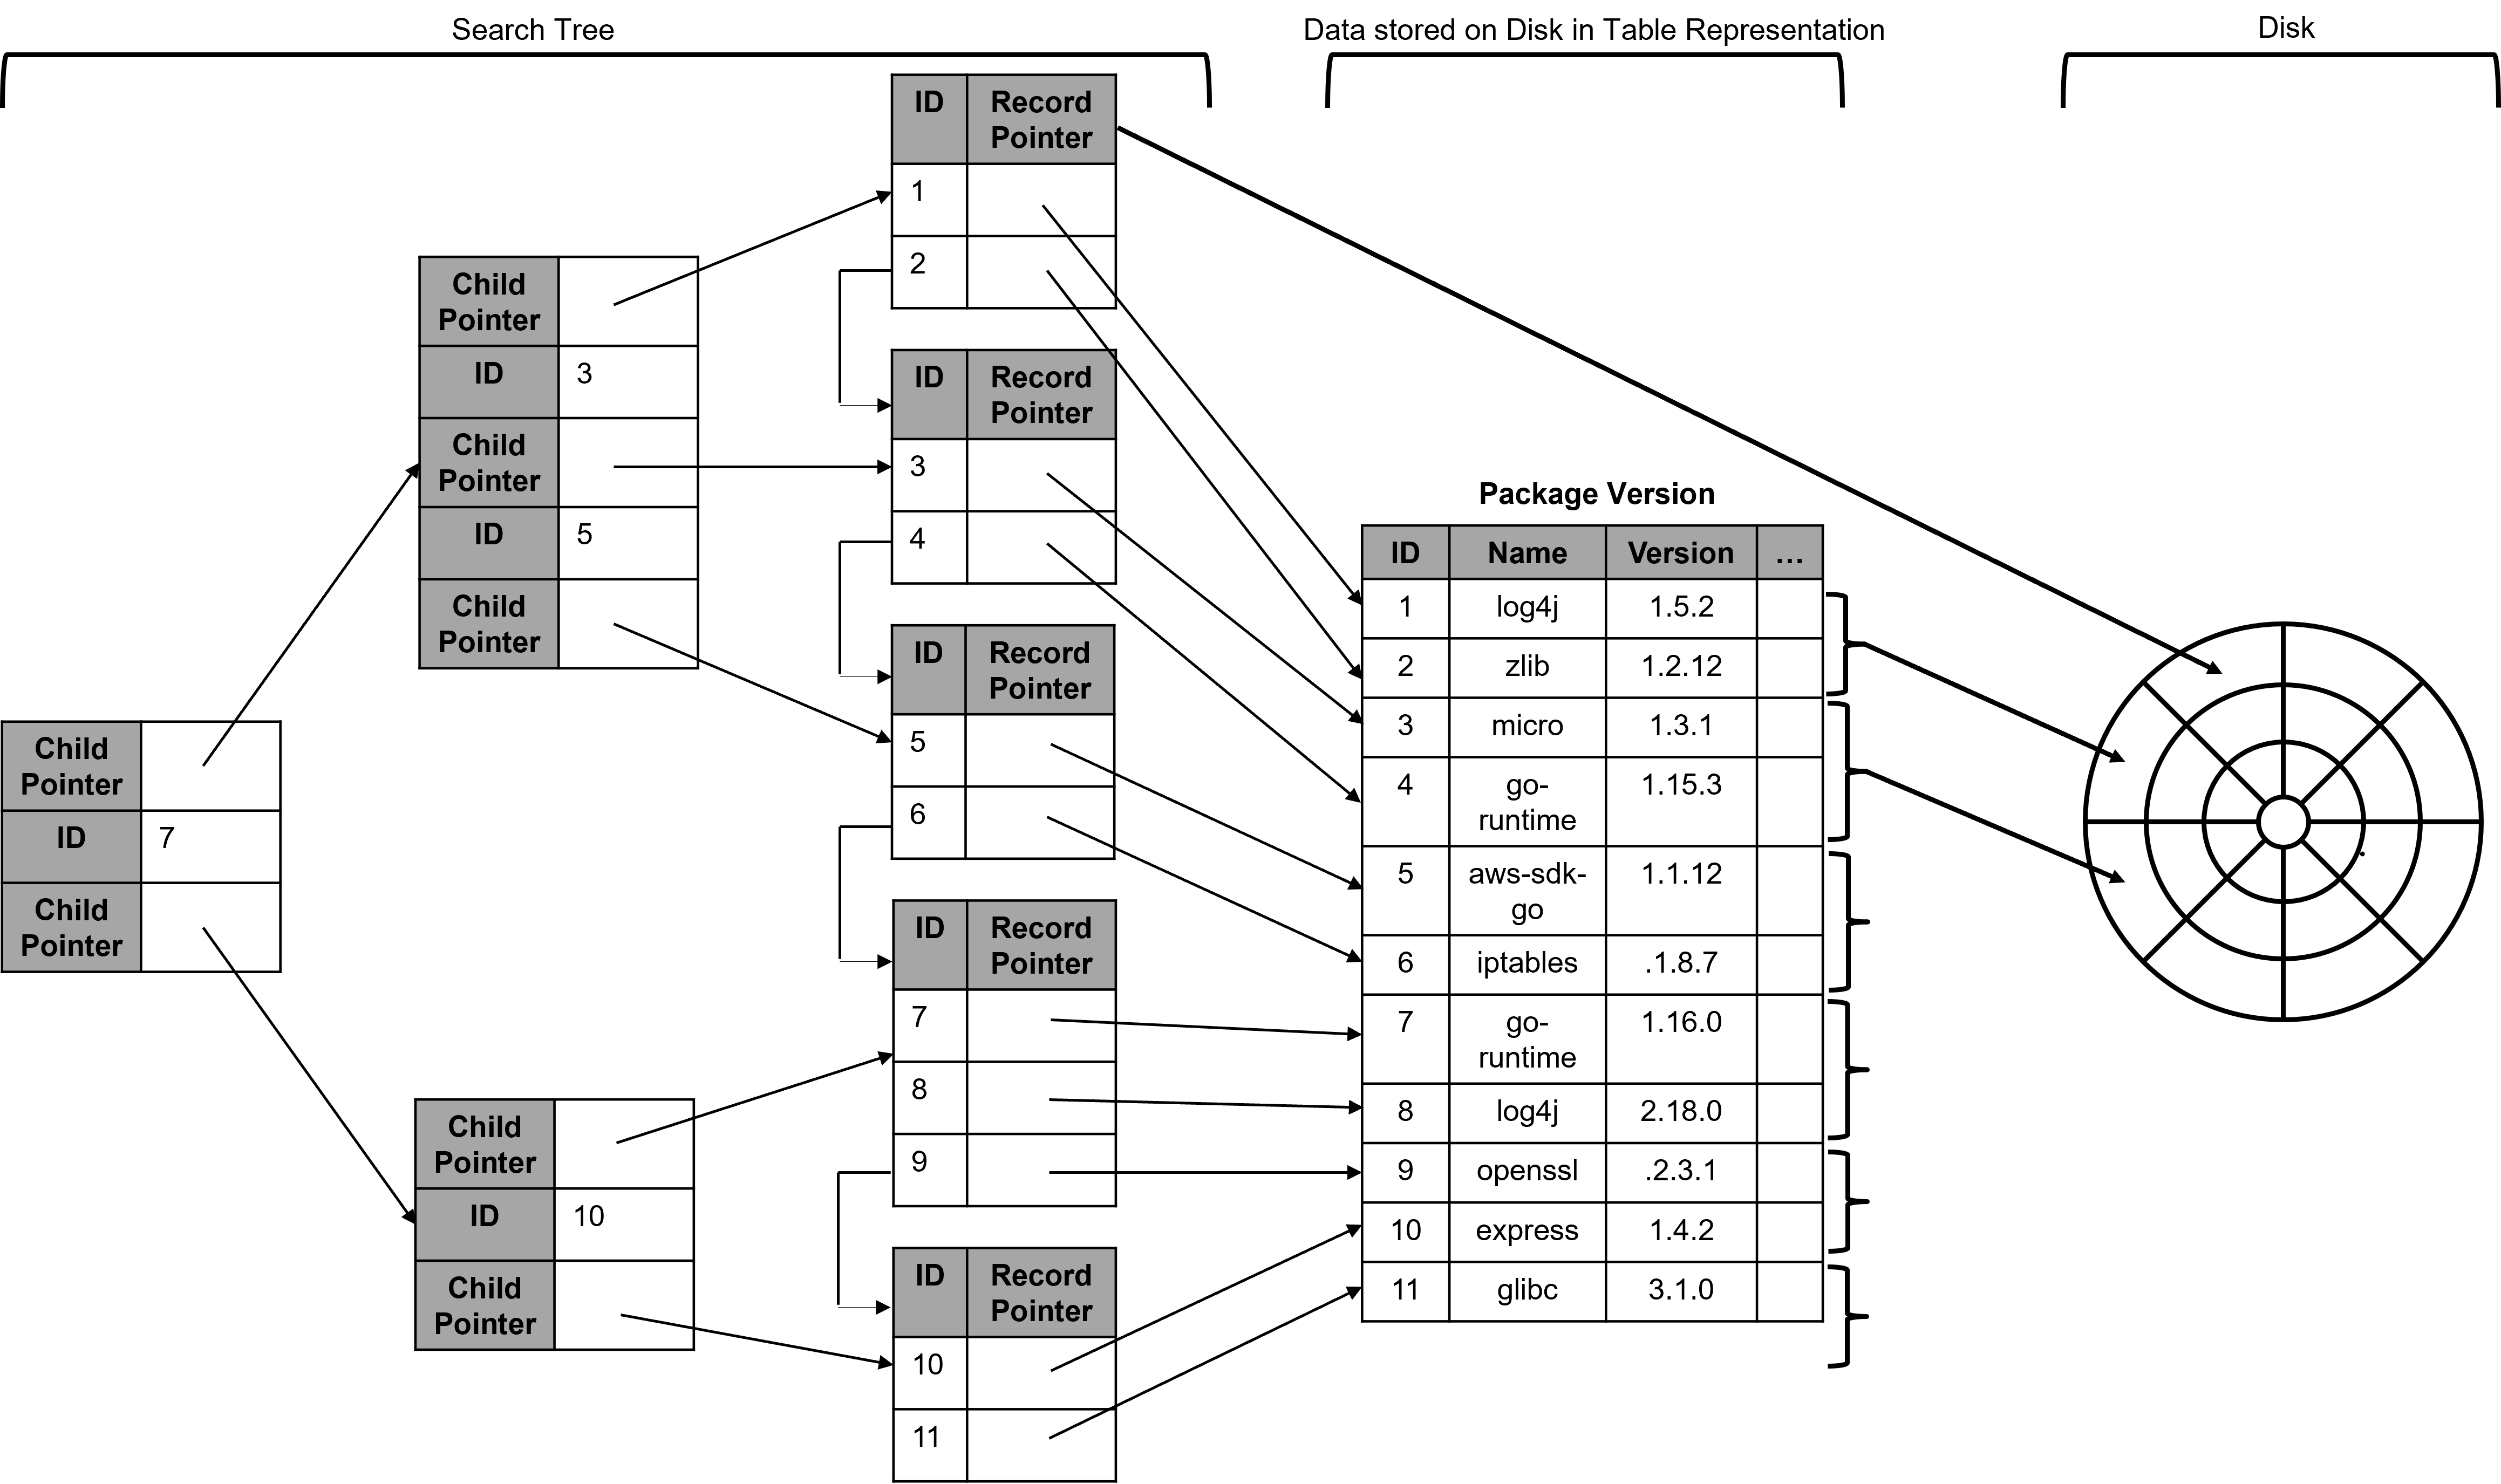
\includegraphics[scale=0.40]{Btree}
	\caption[B\textsuperscript{+}-tree as 4-way Search Tree]{B\textsuperscript{+}-tree as 4-way Search Tree \source{Based on \cite{DatabaseFundamentals}}}
	\label{fig:B+tree}
\end{figure}

So, figure \ref{fig:B+tree} provides a holistic view onto the search trees and how they are used in database systems with some simplifications and assumptions.\par 
On the right of the figure is a representation of a \emph{magnetic disk}, which is still most commonly used as storage for large databases. The concentric circles are called tracks. These tracks are further divided into \emph{sectors}, represented by the intersections of the concentric and straight lines. This division leads to equal-sized \emph{disk blocks}\footnote{One may wonder that these blocks are not equal sized in the figure. The outer ones are actually much larger than the inner ones. In practice, there are different types of sector organization. The type shown in the picture maintains a fixed angle. To provide equal-sized disk blocks nonetheless, the outer sectors usually have a lower record density \cite{DatabaseFundamentals}} which are also commonly called \emph{pages}. The pages are the areas the arrows are pointing to in the figure. With InnoDB, the block size may be configured between 4KB and 64KB.\par 
Data in secondary storage such as a disk cannot be processed directly by the \emph{central processing unit (CPU)}. First, it must be copied into a primary storage such as main memory which is usually \emph{dynamic random access memory (DRAM)}. The units in which this data is transferred between disk and main memory are the just introduced pages. Thus, to read data contained in a certain page, the whole page is copied into the main memory. And to change that data, it is edited and then the whole page is written back, or in other words copied, to the disk. As accessing pages on the disk is in the order of milliseconds while accessing RAM is in the order of nanoseconds, this is a major bottleneck and therefore, the goal is to \emph{minimize the number of block transfers}. So this enables to understand the necessity of \emph{multilevel indexes} or \emph{search trees}.\par
By only looking at figure \ref{fig:B+tree} without the background knowledge just provided, there would be no apparent reason to construct and store such a sophisticated search tree. It would be more efficient to just store the index as a sorted table. Then, when accessing the database with said index, load the whole table into main memory and conduct a binary search. Thus, the only reason to use such search trees is when the index itself outgrows the page size and therefore has to be stored in multiple pages. So, in practice, each node of a search tree is stored in a separate page as indicated by the arrow from the upper index leaf node. By traversing this search tree, the number of necessary page accesses may be reduced significantly. The index size with a search tree of order 4, so a node can at most have 4 children, is probably the most obvious simplification in above figure. The node and leaf indexes are so small that they could easily be stored together in a single index table.\par 
The example shows the search tree as used for secondary file organization. So the records could generally be stored as a heap file, with no ordering at all. If used for primary file organization, instead of having pointers to the actual records, the leaves would directly store the records enforcing a respective order.\par
To traverse such a search tree, for example to find the record with ID 4, one starts at the root node. This is the node illustrated on the far left. As 4 < 7, one follows the pointer above the 7 to the corresponding child node. In practice, this is a pointer to the page of the child node and consequently leads to copying this page into main memory. Then, this process repeats, as 3 < 4 < 5, one follows the pointer between 3 and 5 to the next child node. In this example, this is already a leaf node, containing the pointer to the actual record with ID 4. So here, 4 pages have to be loaded, 3 index pages and the page containing the actual record.\par
So up until now, instead of B-tree or B\textsuperscript{+}-tree, the term search tree was used. This is because B/B\textsuperscript{+}-trees are essentially search trees which have to abide to an extra set of constraints. To be more concrete, a \emph{B-tree of order m} is a tree which satisfies the following properties \cite{SortingSearchingBible}.

\begin{quote}
	\begin{enumerate}
		\item\textit{Every node has at most m children. }
		\item\textit{Every node, except for the root and the leaves, has at least $\lceil m/2 \rceil$ children}
		\item\textit{The root has at least 2 children (unless it is a leaf).}
		\item\textit{All leaves appear on the same level}
		\item\textit{A nonleaf node with k children contains k-1 keys}
	\end{enumerate}
\end{quote}

The goals of \emph{balancing}, which is another term for all leaf nodes being on the same level, is to make the search speed uniform. Thus, the average time to find any random key is roughly the same. Furthermore, these constraints ensure that the nodes stay relatively full and do not end up empty if there are many deletions, thereby preventing the waste of storage space and an unnecessary high number of levels.\par 
Figure \ref{fig:B+tree} shows a B\textsuperscript{+}-tree. A B\textsuperscript{+}-tree is actually a variation of a B-tree which stores record pointers only at the leaf nodes. Consequently, the leaf nodes have an entry for every ID leading to some IDs -- specifically 7, 3, 5 and 10 -- being contained twice in the search tree. On the contrary, in a B-tree every ID is only present once at some level in the tree and the record pointer is stored directly alongside the child pointers. Thus, in above figure, the root node would additionally have a pointer to the record with ID 7. But of course, the whole tree structure would be different, as several leaf nodes could be omitted. Furthermore, B\textsuperscript{+}-trees usually link the leaf nodes to provide ordered access. This is indicated by the the arrows between the leaf nodes. In practice, this linking is also done with an additional pointer \cite{DatabaseFundamentals}.\\

Finally, the \emph{upper bound on running time} for searches with B-trees is examined. Initially, it is important to understand, the leaves carry essentially no information searching wise. Thus, for these considerations, leaves may just be regarded as terminal nodes. As explained in Donald Knuth's ''Art of Computer Programming - Sorting and Searching'' \cite{SortingSearchingBible}, suppose there are \emph{N} keys, and the \emph{N+1} leaves appear on level \emph{l} (In the book the relation that a B-tree with \emph{N} keys always has \emph{N+1} leaves is just given. For a further explanation on why this is always the case, refer to appendix \ref{apx:Relation of Number of Keys and Number of Leaves in a B-tree}). Then, as per constraint, the number of nodes on levels 1,2,3, ... is at least $2$, $2 \lceil m/2 \rceil$, $2 \lceil m/2 \rceil ^2$, ..., hence
$$ N + 1 \geq 2 \lceil m/2 \rceil ^l-1 $$
Solving the equation for l
$$ l \leq 1 + log_{\lceil m/2 \rceil}(\frac{N + 1}{2}) $$
Furthermore, on every level at most $m$ keys have to be searched. As the elements in the nodes of a B-tree are sorted, binary search may be used. Therefore, the maximum number of look ups $s$ per level is $log_2(m)$. Consequently, the total number of look ups is 
$$ s \leq \lceil (1 + log_{\lceil m/2 \rceil}(\frac{N + 1}{2})) \rceil * log_2(m) $$ 
Considering Big $O$ notation, constants may be ignored. Also $m$ is definitely smaller than and independent of $N$. This leads to a worst case time complexity for searching a B-tree of 
$$ O(log N) $$ 
The estimation is also true for B\textsuperscript{+}-trees.\footnote{Although this section covers several details, it is still just a very brief introduction into relational databases, the internals of database systems and B-trees, only covering the topics in the depth necessary for understanding the further sections. Aspects such as transactions and ACID criteria, how the records are actually placed on the disk, how variable-length fields are handled or what happens when records exceed page boundaries have been omitted. Regarding B/B\textsuperscript{+}-trees, the algorithms used for insertion or deletion and their respective bounds on running time are not discussed either. For further and more detailed information on these topics, refer to the respective sources ''The Relational Model for Database Management'' \cite{RelationalDatabaseModel}, ''Fundamentals of Database Systems'' \cite{DatabaseFundamentals} and ''The Art of Computer Programming - Searching and Sorting'' \cite{SortingSearchingBible}.}

\subsubsection{Suitability for the Central Metadata Store}
To evaluate and properly illustrate the suitability of the database technology regarding the aforementioned relevant properties, a representative example based on the established data model is used. The complete data model is quite complex and its actual instantiated form, thus the final entity types, relationships and especially the properties, depends on the use case. Therefore, to keep the considerations general and clear, the representative example only considers the \emph{Package Version} entity type. Since \emph{Package Versions} may be contained in other \emph{Package Versions}, this example allows for considering arbitrarily complex relationship chains.\par

\begin{figure}[H]
	\centering
	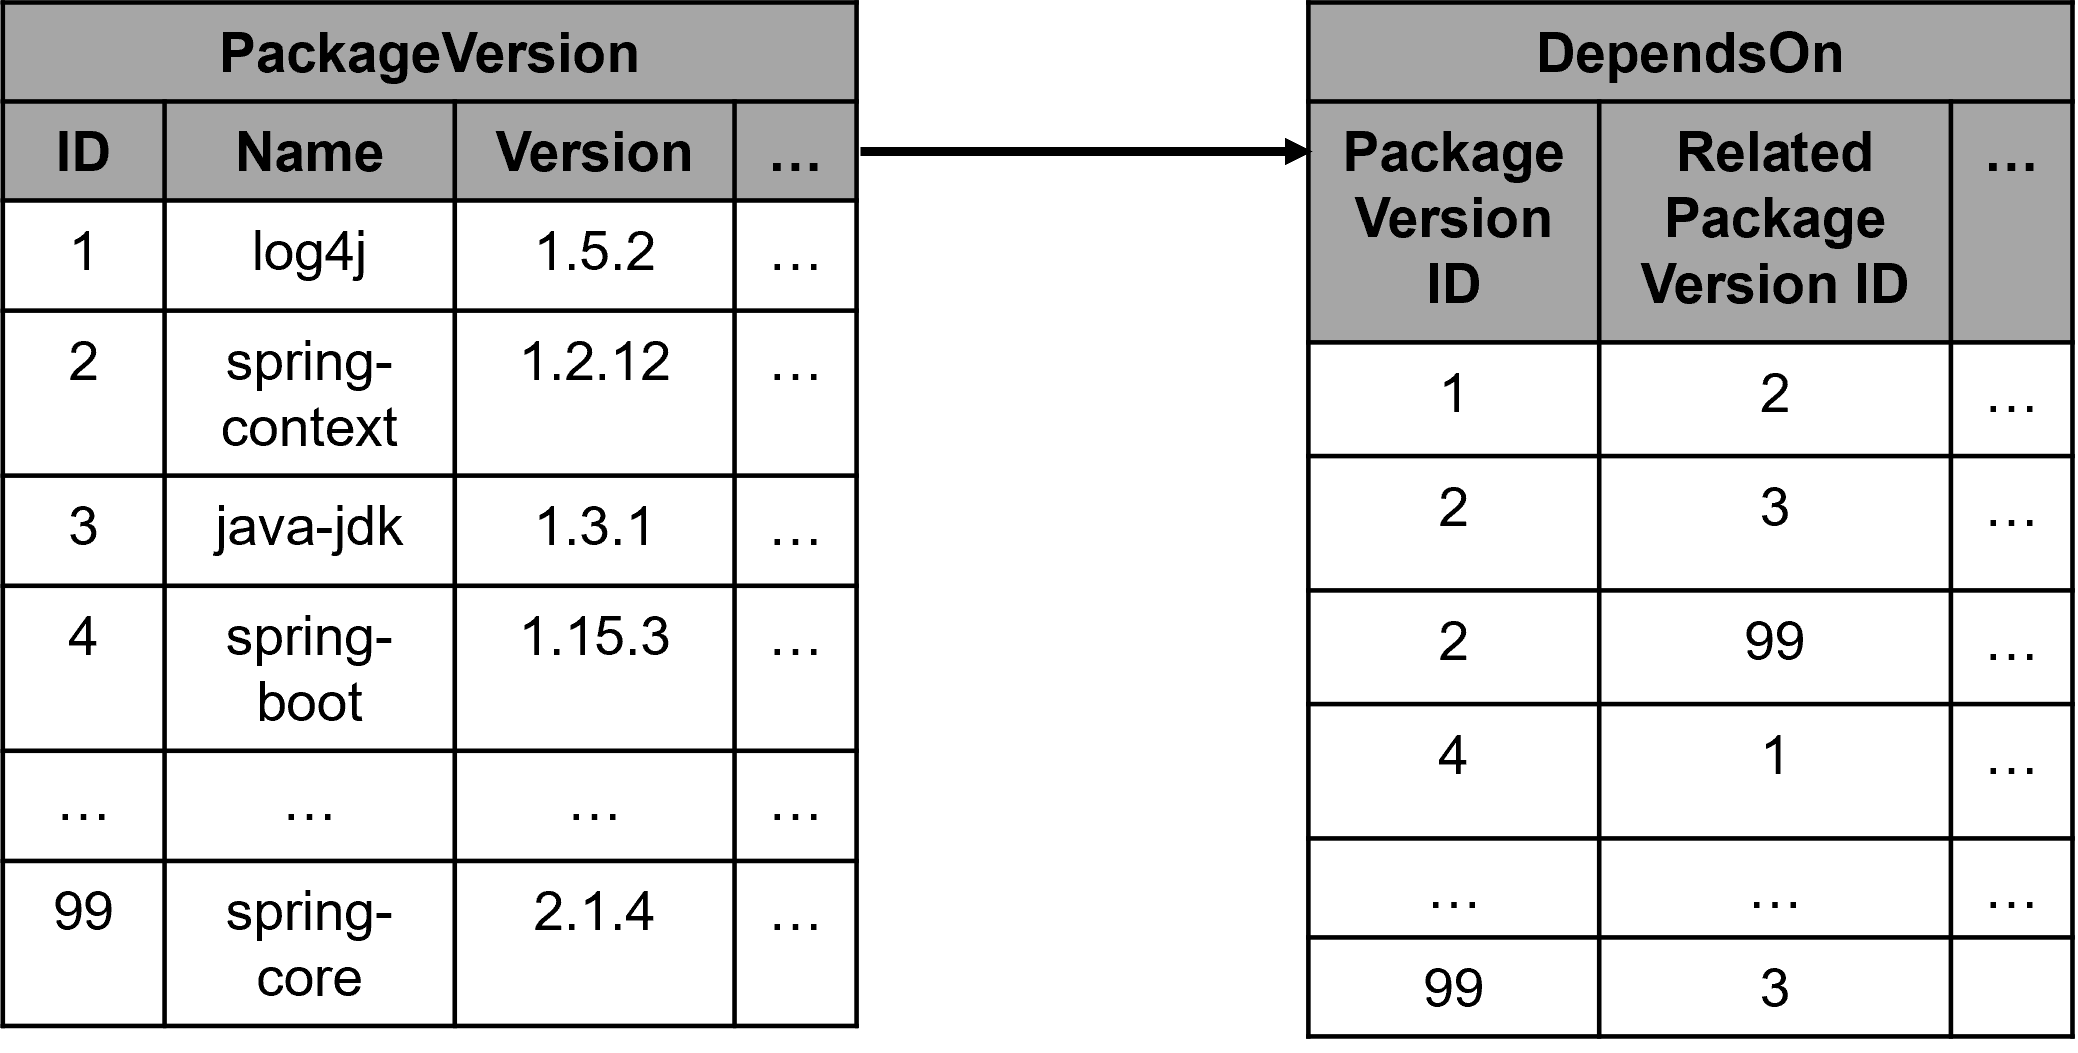
\includegraphics[scale=0.70]{friendsoffriends}
	\caption[Package Versions and Dependencies as Table]{Package Versions and Dependencies \source{Based on \cite{neo4j}}}
	\label{fig:PackageVersionsAndDependencies}
\end{figure}

Figure \ref{fig:PackageVersionsAndDependencies} shows the \emph{Package Version} entity type and the corresponding \emph{depends on} relationship type mapped to tables and filled with some example entities.  As indicated by the ordering of the tables, the example also assumes there are indexes on \emph{ID} and \emph{PackageVersionID}. Furthermore, it may also be assumed, that there is a composite index on \emph{Name} and \emph{Version}.\par
For simplicity reasons, initially pretend there are no transitive dependencies. In this case, to answer the question ''Which Package Versions does the spring-context:1.2.12 Package Version depend on?'' in a relational database, the following SQL query would have to be used:

\begin{lstlisting}[language=SQL, caption=Package Version Dependencies, captionpos=b, label=lst:PackageVersionDependencies]
SELECT p1.Name, p1.Version
  FROM PackageVersion p1 
  JOIN DependsOn
    ON DependsOn.RelatedPackageVersionID = p1.ID
  JOIN PackageVersion p2
    ON DependsOn.PackageVersionID = p2.ID
 WHERE p2.Name = ''spring-context'' AND p2.Version = ''1.2.12''
\end{lstlisting}

Based on the sample data in figure \ref{fig:PackageVersionsAndDependencies}, this returns \emph{java-jdk 1.3.1} and \emph{spring-core 2.1.4} \cite{neo4j}. Although slightly hard to read, the query is still relatively simple and not particularly computationally expensive, because it constraints the number of rows under consideration by applying the filter \lstinline|WHERE p2.Name = ''spring-context'' AND | \lstinline|p2.Version = ''1.2.12''|. Based on the indexes, the initial look up of this record has a time complexity of $O(log(n))$ with $n$ being the number of rows in the \emph{PackageVersion} table. The consecutive join then has a time complexity of $O(m*log(n))$ with $m$ being the number of records found during the previous look up and $n$ being the number of rows in the \emph{DepensOn} table. Each additional join in the query adds a $O(m*log(n))$. This assumes the so called nested loop join algorithm is used. This is usually the most efficient join algorithm in such scenarios, where indexes on the join condition exist and it is a small number of rows that have to be joined. Relational databases automatically estimate and choose the best strategy \cite{PostgreSQLJoin}. Thus, depending on the number of joins, the general time complexity for such a relationship traversal query may be estimated with
$$O(log(n)) + O(m*log(n)) + ... + O(m*log(n))$$ 

Now, to answer the reciprocal question ''Which Package Versions depend on the spring-context:1.2.12 Package Version?'' in a relational database, the following SQL query would have to be used:

\begin{lstlisting}[language=SQL, caption=Package Version Reciprocal Dependencies, captionpos=b, label=lst:PackageVersionReciprocalDependencies]
SELECT p1.Name, p1.Version
  FROM PackageVersion p1 
  JOIN DependsOn
    ON DependsOn.PackageVersionID = p1.ID
  JOIN PackageVersion p2
    ON DependsOn.RelatedPackageVersionID = p2.ID
 WHERE p2.Name = ''spring-context'' AND p2.Version = ''1.2.12''
\end{lstlisting}

Based on the sample data in figure \ref{fig:PackageVersionsAndDependencies}, this returns \emph{log4j 1.5.2} \cite{neo4j}. Although this query looks very similar to the one before, it is computationally more expensive, because there is no index on \emph{RelatedPackageVersionID} and consequently, the whole table has to be considered for the join with a complexity of $O(n)$. In practice, an additional index could be added without problems, as the write performance which would suffer from maintaining an additional index, does not matter too much in this use case. Then joining each record would also have a complexity of $O(log(n))$, leading to the same overall complexity as the previous query.\\

Finally, the transitive dependencies have to be considered. To traverse these transitive dependencies in SQL, recursive joins have to be used. Therefore, joining a table with itself. But as the dependency chains may be of arbitrary length, a simple recursive query is not sufficient. Nowadays, most of the popular relational databases provide a SQL feature, the WITH clause, or rather \emph{Common Table Expressions (CTE)}, to support recursive queries \cite{mysqlCTE, postgresCTE, sqliteCTE}. CTEs are auxiliary statements which can be thought of as defining temporary tables existing for just one query \cite{postgresCTE}. So, to actually answer the question ''Which Package Versions does the spring-context:1.2.12 Package Version depend on?'' correctly, thus also including the transitive dependencies, the following SQL query would have to be used:

\begin{lstlisting}[language=SQL, caption=Package Version Dependencies (including transitive), captionpos=b, label=lst:PackageVersionDependenciesIncTransitive]
WITH RECURSIVE cte(PackageVersionID) AS (
  -- Anchor member.
  SELECT d.RelatedPackageVersionID
    FROM DependsOn d
    JOIN PackageVersion p
      ON d.PackageVersionID = p.ID
   WHERE p.Name = 'spring-context' AND p.Version = '1.2.12'
  UNION ALL
  -- Recursive member.
  SELECT d.RelatedPackageVersionID
    FROM DependsOn d
    JOIN cte
      ON d.PackageVersionID = cte.PackageVersionID
)

SELECT p.Name, p.Version
  FROM PackageVersion p
  JOIN cte
    ON cte.PackageVersionID = p.ID
\end{lstlisting}

Based on the sample data in figure \ref{fig:PackageVersionsAndDependencies}, this returns \emph{java-jdk 1.3.1} twice (as union all does not remove duplicates) and \emph{spring-core 2.1.4}. And correspondingly to answer reciprocal question ''Which Package Versions depend on the spring-context:1.2.12 Package Version?'', the following SQL query would have to be used:

\begin{lstlisting}[language=SQL, caption=Package Version Reciprocal Dependencies (including transitive), captionpos=b, label=lst:PackageVersionReciprocalDependenciesIncTransitive]
WITH RECURSIVE cte(PackageVersionID) AS (
  -- Anchor member.
  SELECT d.PackageVersionID
    FROM DependsOn d
    JOIN PackageVersion p
      ON d.RelatedPackageVersionID = p.ID
   WHERE p.Name = 'spring-context' AND p.Version = '1.2.12'
  UNION ALL
  -- Recursive member.
  SELECT d.PackageVersionID
    FROM DependsOn d
    JOIN cte
      ON d.RelatedPackageVersionID = cte.PackageVersionID
)

SELECT p.Name, p.Version
  FROM PackageVersion p
  JOIN cte
    ON cte.PackageVersionID = p.ID
\end{lstlisting}

Based on the sample data in figure \ref{fig:PackageVersionsAndDependencies}, this returns \emph{log4j 1.5.2} and \emph{spring-boot 1.15.3}. The queries are tested with a PostgreSQL 15 database. The respective DDL statements to set up the sample data are included in appendix \ref{apx:Data Definition Statement for SQL Sample Data}.\par
Besides the computational complexity and the general difficulty of the queries, another aspect to consider are the \emph{schemas} required by relational databases. This may lead to a lot of null values in a table in cases where data sources do not provide the same amount of information for entities of the same type. Depending on how the data is stored on disk, this may lead to a waste of storage space. But most importantly, by \emph{enforcing a schema on database level}, the flexibility to store further raw data provided by the data sources is lost. Furthermore, this makes it difficult to create or adjust schemas at application runtime. This is an issue for a central metadata store, considering that the properties and even several entities depend on the specific component model, data sources and also the use case.\\

So, as a conclusion for this section, a quick summary of the most important aspects when considering a relational database for the use case. 
(n:m)-relationships lead to large tables in relational databases. To be able to efficiently traverse these relationships and run queries with a reasonable performance, it is important to define \emph{indexes} on the columns used in the respective join conditions. Relational databases that support recursive CTEs are able to \emph{traverse hierarchies of arbitrary depth} without additional logic in the client side code. The \emph{queries to traverse several relationships become quite large and may be hard to read}. The necessity for a schema on database level leads to a considerable loss of flexibility. 
 
\subsection{Document Databases}
\emph{Document Databases} have grown tremendously in popularity throughout the last several years. Especially MongoDB which is ranked the top 4 most used database in Stack Overflow's 2021 developer survey has found widespread use as a primary database for applications and therefore, as a substitute for relational databases \cite{StackoverflowDeveloperSurvey}.

\subsubsection{Theoretical Foundation}
Document databases are a type of NoSQL database which is commonly interpreted as an acronym for ''Not only SQL''. It is thereby somewhat of an extension of the most simplistic kind of databases, the \emph{key-value databases}. These enable very fast look ups at the cost of only allowing users to address records by their key. The value is usually \emph{opaque} to the database. Correspondingly, document databases also do not require a schema for the values they store, but they store the values in a standard format such as XML, PDF or most frequently JSON \cite{NoSQL}. Hence, the values are not opaque and the database may still parse the data and create indexes on non-key fields even though being \emph{schema-less}.\\

Generally, the primary reason for using document databases, or rather any NoSQL databases, are the horizontal scalability issues of relational databases \cite{NoSQL}. While vertical scalability refers to providing the database machine with more compute resources, thus, CPU and RAM, horizontal scalability refers to distributing the database over multiple machines. The relevant questions at this point are: Where do the scalability issues come from? How are they overcome by document databases?\par
\emph{De-normalization} is one of the key features of document databases. Thus, while relational databases map entity types and relationships to multiple tables connected by foreign keys, document databases allow storing entities and relationships as nested structures through their schema-less nature. These nested structures are often referred to as \emph{documents} or also more generally \emph{aggregates}, a term from \emph{Domain-Driven Design} describing a collection of related objects that is treated as a unit. Documents are grouped to \emph{collections}, which is kind of the equivalent to a table in relational databases \cite{NoSQLDistilled}. A common example is shown by figure \ref{fig:NoSQLDataModel} and listing \ref{lst:JSONDocument}.\par 

\begin{figure}[H]
	\centering
	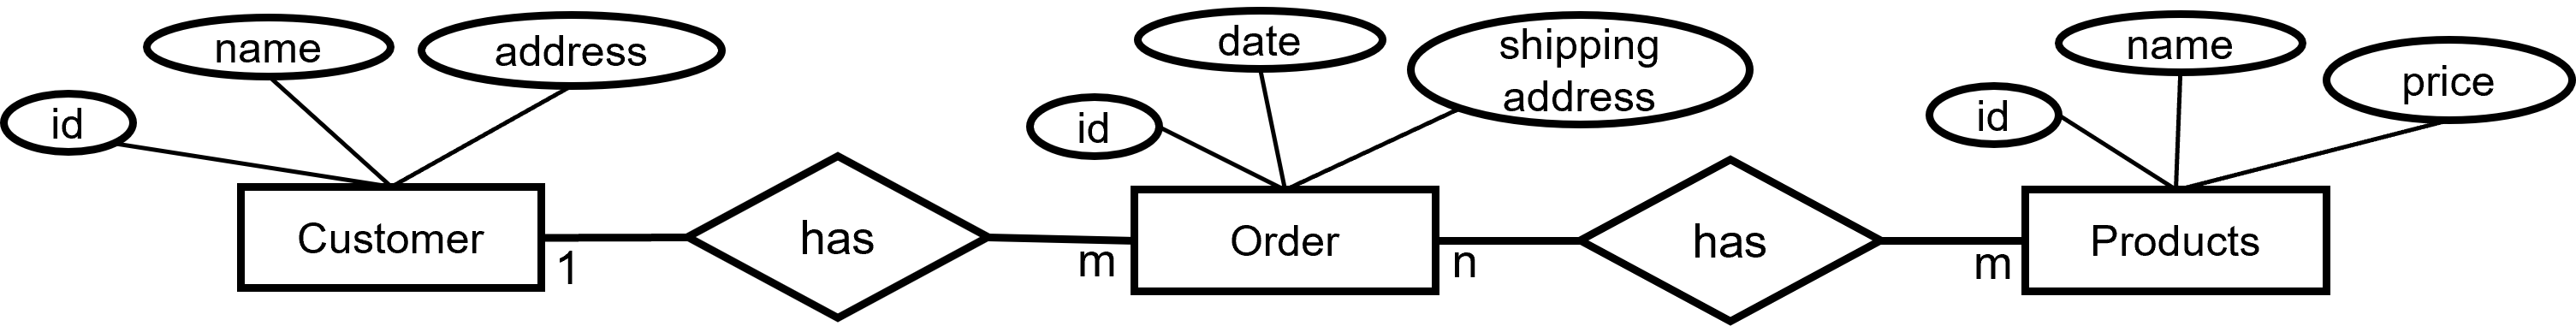
\includegraphics[scale=0.60]{no_sql_datamodel}
	\caption[Sales Data Model]{Sales Data Model \source{Based on \cite{NoSQLDistilled}}}
	\label{fig:NoSQLDataModel}
\end{figure}

\begin{lstlisting}[language=JSON, caption=JSON Document, captionpos=b, label=lst:JSONDocument]
{
  ''id'': 1,
  ''name'': ''Martin'',
  ''address'': 
    {''city'': ''Berlin''}
  ''orders'': [
    {''id'': 99,
     ''date'': ''04.01.2023'',
     ''shippingAddress'': {''city'': ''Berlin''}
     ''products'': [
       {''id'': 42,
        ''name'': ''The Hitchhiker's Guide to the Galaxy'',
        ''price'': 7.50 },
       {''id'': 12,
        ''name'': ''The Art of Computer Programming'',
        ''price'': 120.00 }
      ]
    }
  ]
}
...
\end{lstlisting}


This solves the so called \emph{impedance mismatch}, the difference between the relational model and in-memory data structures. Hence, with relational databases developers frequently have to translate the nested in-memory data structures to a relational representation to persist them. Of course, there are object-relational mapping frameworks such as Hibernate, but these often lead to performance issues \cite{NoSQLDistilled}. By allowing to store objects as JSON objects, document databases such as MongoDB enable developers to store and retrieve their \emph{JavaScript} objects or \emph{Python} dictionaries as they are, without any further conversion. This is definitely one of the major reasons for their success, also in use cases where scalability is not a primary concern.\par
Furthermore, through this de-normalization, document databases \emph{remove the necessity of joining a lot of data}. On one hand, this makes querying objects such as customer with all its orders easier for developers, as join queries are comparably difficult to write and understand. On the other hand, this increases the performance and scalability of these queries, as joins add quite some computational complexity which even depends on the number of stored objects. Thus, the performance of joins becomes worse as the database grows.\par
Besides, this kind of data organization enables efficient \emph{sharding}. Sharding is a technique where different parts of the data are put onto different severs. Tables, or in the context of document databases rather collections, are split up into smaller shards which may be placed on multiple servers. A common sharding technique is to hash a key, also called \emph{shard key} in MongoDB \cite{MongoDBShardKey} or \emph{partition key} in DynamoDB \cite{DynamoDBPartitionKey}. The respective hash value determines where, so on which server, to place the shard. This hashing provides an even distribution. But there are also other techniques such as ranged sharding. Thereby, the shards are distributed by the key value itself. This may be useful, when the records have some sort of order and it is common to access multiple sequential records. Or the key may be a post code and the distribution is based on the sever location to minimize latency \cite{NoSQLDistilled}. This whole technique is enabled through the nesting, as documents are collection of related objects that are treated as units. Therefore sharding, or generally any form of partitioning, is rather difficult with relational databases. Since the data is scattered over multiple tables and the query language SQL puts no restrictions on how to query and connect this data, such partitioning would regularly require to send requests over the network to collect all the information \cite{NoSQLDistilled}.\par 
So de-normalization obviously has numerous advantages. And this is also where most getting started guides of document databases such as MongoDB stop \cite{MongoDBGettingStarted}. But naturally, it introduces the issues which were solved by normalization in the first place. Considering the example above, there is a (n:m)-relationship between orders and products. As the product is nested in the order which is again nested within the customer, updating a particular product while maintaining data integrity requires searching through all customers and through all orders within those customers, to update every single occurrence. Of course, in some cases write performance may not be relevant. But the nesting also affects queries. Imagine the above example describes the database of a retailer and this retailer wants to analyze its ''Hitchhiker's Guide to the Galaxy'' product sales over the last year. Again, to do this, the database has to search through all orders within all customers. There is the option to create indexes on nested fields which works pretty similar to relational database indexes to increase this performance. The problem that remains in this case is that document databases still have to retrieve the entire documents that contain the respective product from disk, thus, every customer record with all orders and all products. This leads to enormous RAM usage and may also slow down the performance significantly \cite{MongoDBAppliedDesign}.\\\\
Generally, there are several restrictions which may serve as an orientation whether to nest or embed documents or whether to normalize and link them. \par 
If the application frequently has to \emph{access the embedded document independently of the embedding document(s)} and the \emph{documents are quite large}, it may be best to normalize and link the document rather than embedding due to the otherwise excessive RAM usage \cite{MongoDBAppliedDesign}. In above example, orders may be queried independently of customers. So it may be better to normalize this and make the orders reference the respective customer.\par 
\emph{If documents grow, the database may have to relocate it on disk} to an area with more space. In the above example, as a customer may regularly order products from the retailer, the order array within the customer document would grow and potentially require relocation. Such a relocation decreases performance significantly \cite{MongoDBAppliedDesign}. Moreover, document databases may even have a \emph{hard limit for the document size}. For MongoDB, this limit is 16MB \cite{MongoDBDocumentSizeLimit}. So, this is another argument to normalize the orders.\par 
Considering all these limitations, many-to-many relationships are especially problematic to de-normalize. Therefore, MongoDB even suggests to \emph{model complex many-to-many relationships in normalized form} \cite{MongoDBDataModeling}. For simple many-to-many relationships, where the references may rarely be updated, it is also a possibility to embed the references instead of creating the equivalent of a join table.\par
As especially MongoDB and its query language provide a lot of the functionality also provided by SQL, the final question may be, why not store the relational model in a document database? The primary concern therefore may be data integrity. Although MongoDB provides ACID conform transactions, there is no way to enforce referential integrity on database level. Without a database schema, there is no way to tell the database about foreign keys and corresponding constraints.\par Furthermore, several operations such as joining are usually more efficient with a relational database. The syntax to perform the join is also simpler with SQL. To make this more tangible, below listing shows the syntax to perform the logical equivalent to a left outer join on orders with products. The example thereby assumes the data is stored according to a relational model as shown in appendix \ref{apx:Data Definition Statement for MongoDB Sample Data}. 

\begin{lstlisting}[language=JSON, caption=JSON Document, captionpos=b, label=lst:JSONDocument]
db.orders.aggregate([
{ ''$match'': { ''_id'': 1 } },
{ ''$lookup'': {
  ''from'': ''relations'',
  ''let'': { ''orderId'': ''$_id'' },
  ''pipeline'': [{''$match'':{''$expr'':{''$eq'':[''$order'',''$$orderId'']}}},
  { ''$lookup'': {
    ''from'': ''products'',
    ''let'': { ''productId'': ''$product'' },
    ''pipeline'': [{''$match'':{''$expr'':{''$eq'':[''$_id'',''$$productId'']}}}],
    ''as'': ''products'' }
  }],
  ''as'': ''order_products'' }
},
{ ''$project'': {
  ''_id'': 1,
  ''date'': 1,
  ''shippingAddress'': 1,
  ''products'': ''$order_products.products'' }
}
])
\end{lstlisting}

Without going into too much detail about this query, it is obvious that it is rather complex and resembles a query execution plan. Thereby, the output of each stage (\$match, \$lookup, \$lookup, \$project) is the input of the consecutive stage \cite{MongoDBAggrPipeline}. This drastically limits the automatic optimization capabilities. So MongoDB will generally always perform a nested loop join even without indexes when a relational database would probably perform a merge or hash join.\\\\ 
So document databases and de-normalization work especially well, in cases where the application only requires a limited set of specific repetitive access patterns. But in order to actually leverage the advantages, these access patterns have to be identified and the de-normalization has to be done accordingly. This requires a very good understanding of the application already in the data modeling phase.\footnote{Again, although this section covers several details about document databases, it is still just a very brief introduction to provide the foundations necessary for understanding the further sections. Especially the topics of transactions and ACID criteria as well as the CAP theorem and the general treatment of consistency in document databases have been omitted.} 

\subsubsection{Suitability for the Central Metadata Store}
In contrast to the corresponding section about the suitability of relational databases, this one is kept short. Based on the background knowledge provided in the theoretical foundations, it is apparent that the advantages of document databases may barely be leveraged for this use case. Extensive examples on how to implement the central metadata store with the capabilities of a document database are therefore omitted as well.\\\\ 
The data model is based on (n:m)-relationships. Also, the database's primary purpose is to perform analysis about different entities. Thus, ''Which Component Versions contain a vulnerable Log4j Package Version?'' with Package Version being the access point. Or reciprocal, ''Which Package Versions are contained in a particular Component Version?'' with Component Version being the access point. So, there is not a limited set of specific repetitive access patterns as every entity may need be used as access point to answer common questions. Therefore, the \emph{central metadata store cannot really be optimized through de-normalization}.\par
Consequently, at least concerning the major entities, the data model would have to be stored as a relational model. In this case, the document database would have the same scalability issues as relational databases and thereby mitigate a lot of the general advantages of document databases. Relational databases are practically designed with the primary purpose of handling relational models. Consequently, the query language, SQL, as well as the general data processing is better adjusted to such use cases.\par 
But, being \emph{schema-less} on database level may be an advantage. Although there is no way to enforce referential integrity on database level, enforcing a schema on application level allows for easier creation and adjustments at application runtime.

\subsection{Graph Databases}
The last database technology analyzed are \emph{graph databases}. They are also a type of NoSQL database. Although especially Neo4j is doing a lot of advertising, graph databases are still the least known database technology, as also represented by their absence in Stack Overflow's 2021 developer survey \cite{StackoverflowDeveloperSurvey}.

\subsubsection{Theoretical Foundation} \label{sec:GraphDB Theoretical Foundation}
Again, first a quick repetition of the foundations. The mathematical definition of a graph is the following: 
\begin{quote}
	\textit{A graph is a pair of sets $G = (V,E)$. In an undirected graph, the elements of $E$ are 2-element subsets $\{v,w\}$ of $V$. In a directed graph, the elements of $E$ are 2-element tuples $(v,w)$, thus ordered pairs, of $V$.}
	\cite{IntroductionToAlgorithms}
\end{quote}
In this definition, $V$ refers to \emph{vertices}, or rather \emph{nodes}, and $E$ refers to \emph{edges}. Quite frequently, two nodes $v$ and $w$ connected through an edge $(v,w)$ are elements of different sets, thus, $v \epsilon S1$ and $w \epsilon S2$ with $V = S1 \cup S2$. So, $E$ is a subset of the Cartesian product of $S1 x S2$. Looking back at the definition of relations in section \ref{sec:Theoretical Foundations Relational Database} ''Theoretical Foundations'' of relational databases, this is also the definition of a relation.\par
Thus, $E$ is a \emph{relation} and $V$ is the union of the \emph{source set} and \emph{destination set}. Now, this is generally well known from functions, which are defined by a \emph{domain} $S1$, a \emph{codomain} $S2$ and a \emph{mapping} $f$, which assigns elements of $S1$ to elements of $S2$. Hence, drawing a function in a coordinate system is essentially the visualization of a graph, where commonly the \emph{x-axis} denotes the \emph{source set} and the \emph{y-axis} denotes the \emph{destination set} and the dots, or rather line, for most common functions denotes the \emph{relation}.\par
In practice with business data, the source set and the destination set are usually sets of discrete and finite elements and the relationship between them is rather artificial and application specific. A primitive example, $S1$ may be the set of all package names, $S2$ may be the set of all version numbers and the relation $E$ $(v, w)$ may be package versions. Thereby, the source set and destination set are rather irrelevant. Besides, one could argue that for the scope of an application, the union of all $v$ in $E$ is equal to the source set and the union of all $w$ in $E$ is equal to the destination set.

\begin{figure}[H]
	\centering
	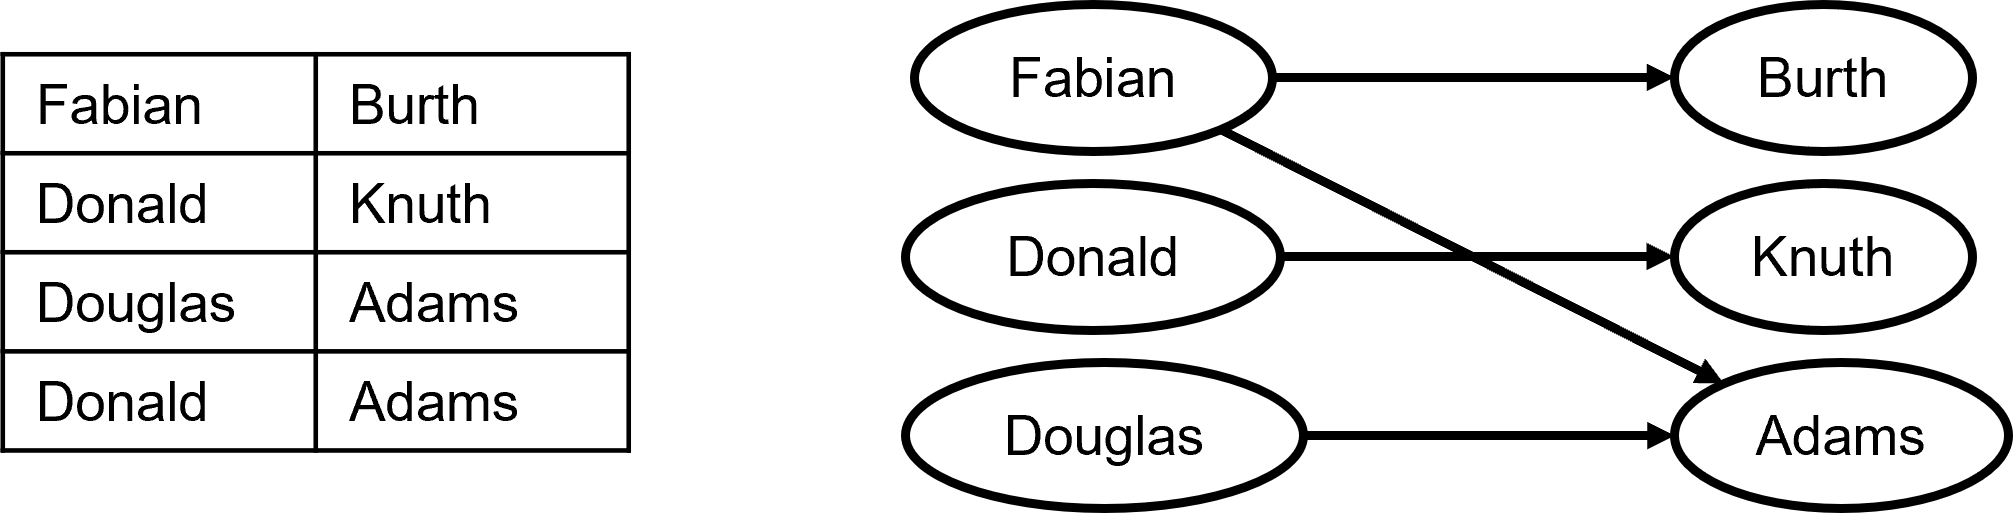
\includegraphics[scale=0.70]{table_vs_graph}
	\caption[Graph Representations]{Graph Representations \source{Own Representation}}
	\label{fig:GraphTheoryExample}
\end{figure}

So, for the scope of an application, the table and the vertices and edges in figure \ref{fig:GraphTheoryExample} may be interpreted as two different representation of the same graph. This comparison of relations and graphs may be a slightly abstract and the example is oversimplified, but its purpose is to show how these two concepts and their common representations are tightly coupled.\\

The first part approached the topic from a mathematical perspective. From here on, this shifts to the actual technologies. Although the previous example may indicate this, in graph databases the graph is not used as a different representation for classical relations, hence to represent the relation of the properties of an entity. It is rather used to represent the relationships between the different entities. Thus, even though figure \ref{fig:GraphTheoryExample} is theoretically accurate, the following figure \ref{fig:GraphDBExample} is more suitable from a database technology perspective.

\begin{figure}[H]
	\centering
	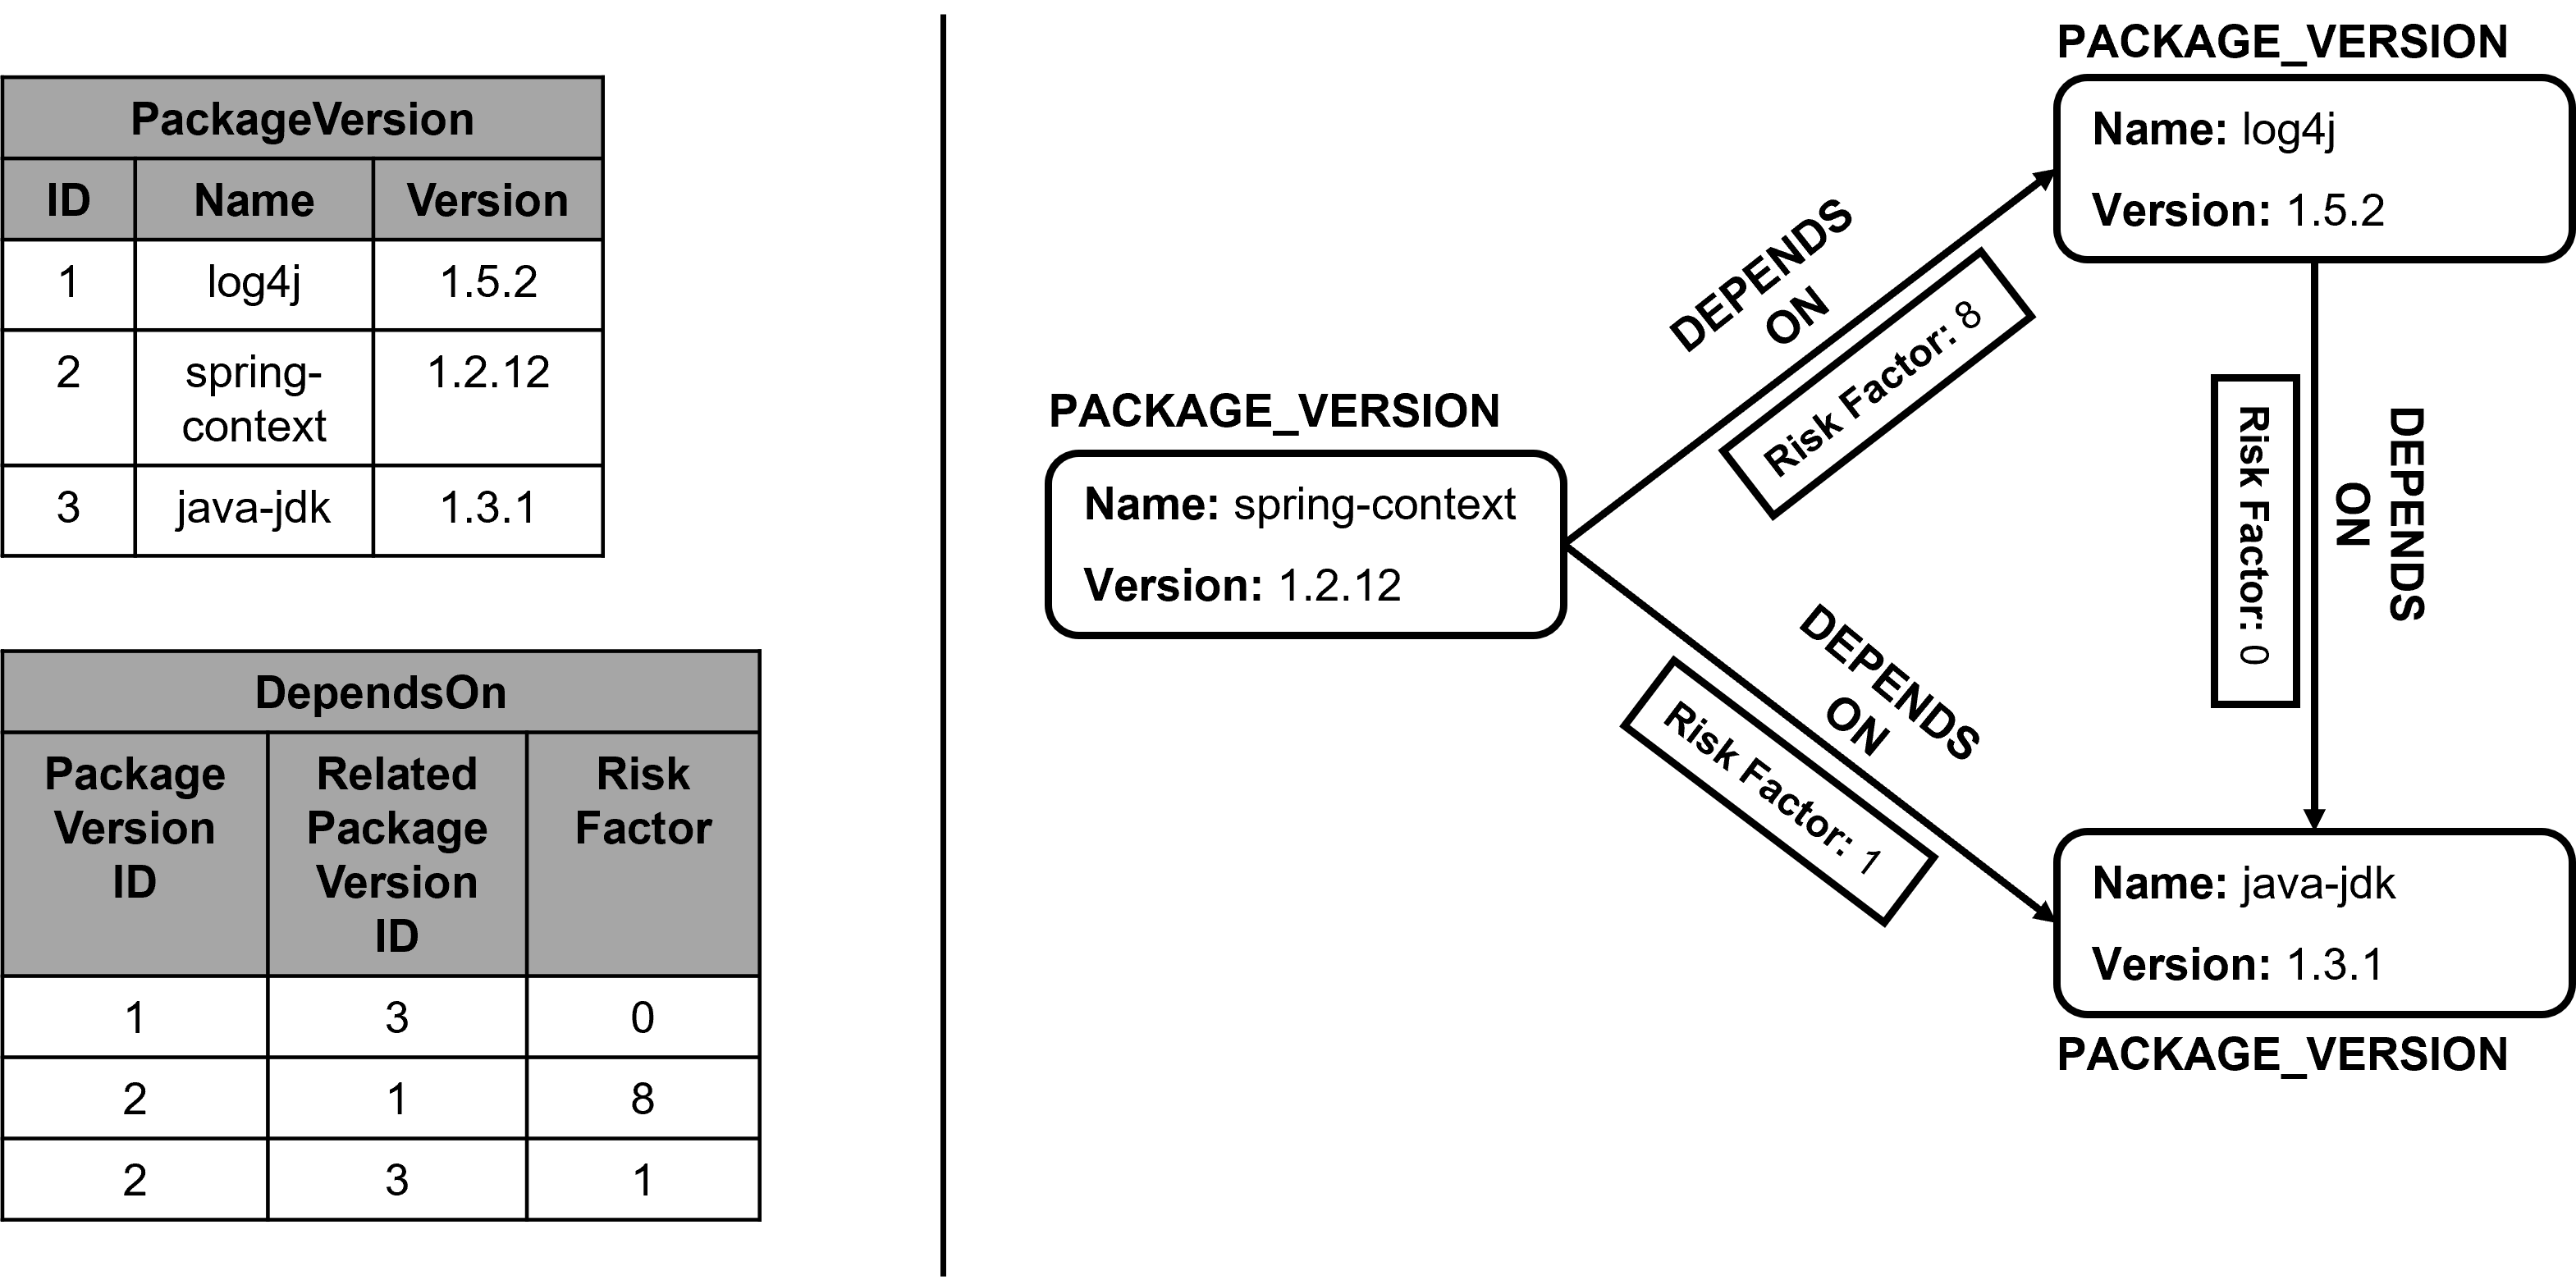
\includegraphics[scale=0.60]{graphdb}
	\caption[Graph Database Representation]{Graph Database Representation \source{Own Representation}}
	\label{fig:GraphDBExample}
\end{figure}

This graph model is called \emph{labeled property graph}. As defined in the ''Graph Databases - New Opportunities for Connected Data'' written by engineers of the Neo4j database, a labeled property graph has the following characteristics \cite{neo4j}:

\begin{quote}
	\begin{enumerate}
		\item\textit{It contains nodes and relationships. }
		\item\textit{Nodes contain properties (key-value-pairs). }
		\item\textit{Nodes can be labeled with one or more labels. }
		\item\textit{Relationships are named and directed, and always have a start and end node. }
		\item\textit{Relationships can also contain properties. }
	\end{enumerate}
\end{quote}

This model is generally quite intuitive. But obviously, even in this more complex example, with the suitable interpretation of the table (thus, instead of interpreting the relation itself, the foreign key relationships are considered), it still expresses the same graph as the nodes and relationships. And, as discussed previously, document databases are able to express this graph as well, either also through a normalized model or through nested documents.\\\\ 
\emph{So the key difference of graph databases is not that they store graphs in general. The key difference is that their file organization and data processing is optimized to work with graph data.}\par
As shown in figure \ref{fig:GraphDBExample} on the bottom left, table representations and consequently relational databases use an index to link entities, or in this context rather nodes. To increase the performance of reciprocal queries, an additional index may be created on \emph{Related Package Version ID}. These \emph{indexes are global}, so as the graph grows, so do the indexes.\par 
In contrast, in most graph databases with native processing capabilities each node maintains direct references to link nodes. Thus, each node maintains kind of a \emph{local index} whose size and consequently performance do not depend on the total size of the graph. This concept of linking adjacent nodes is commonly referred to as \emph{index-free adjacency}.\footnote{There has been a lot of discussion whether index-free adjacency is a requirement for graph databases \cite{graphdbdiscussion}. The current consensus seems to be that it is not, since especially ArangoDB developed another approach to the problem which allows similar complexities as index-free adjacency for traversing graphs \cite{arangodbhybridindexes}.} For further assumptions and explanations, the architecture of the Neo4j database is considered \cite{neo4j}.\par
So, when querying ''Which Package Versions does the spring-context:1.2.12 Package Version depend on?'', the initial look up works quite similar as in relational databases and therefore still has a complexity of $O(log(n))$. But finding the related packages is $O(1)$ instead of $O(log(n))$. Since nodes maintain references to nodes with incoming as well as to nodes with outgoing relationships, the reciprocal query ''Which Package Versions depend on the spring-context:1.2.12 Package Version?'' may be answered with the exact same complexity \cite{neo4j}.\par 
So given these complexities, in theory graph databases scale and perform better than other database technologies when the application involves a lot of graph traversals.\footnote{As before, this theoretical foundation chapter is obviously not complete. Especially the file organization which enables the fast traversals are an interesting topic. For a good and thorough explanation of a implementation, refer to ''Graph Databases - New Opportunities for Connected Data'' \cite{neo4j}.}

\subsubsection{Suitability for the Central Metadata Store}
This suitability section takes a similar approach as the first one, evaluating the suitability of the relational database. Thus, examining the same representative \emph{Package Version} example. This allows for a direct comparison afterwards. Below figure \ref{fig:PackageVersionsAndDependenciesGraph} therefore illustrates the equivalent example from \ref{sec:Theoretical Foundations Relational Database} ''Theoretical Foundations'' of relational databases as a classical graph.

\begin{figure}[H]
	\centering
	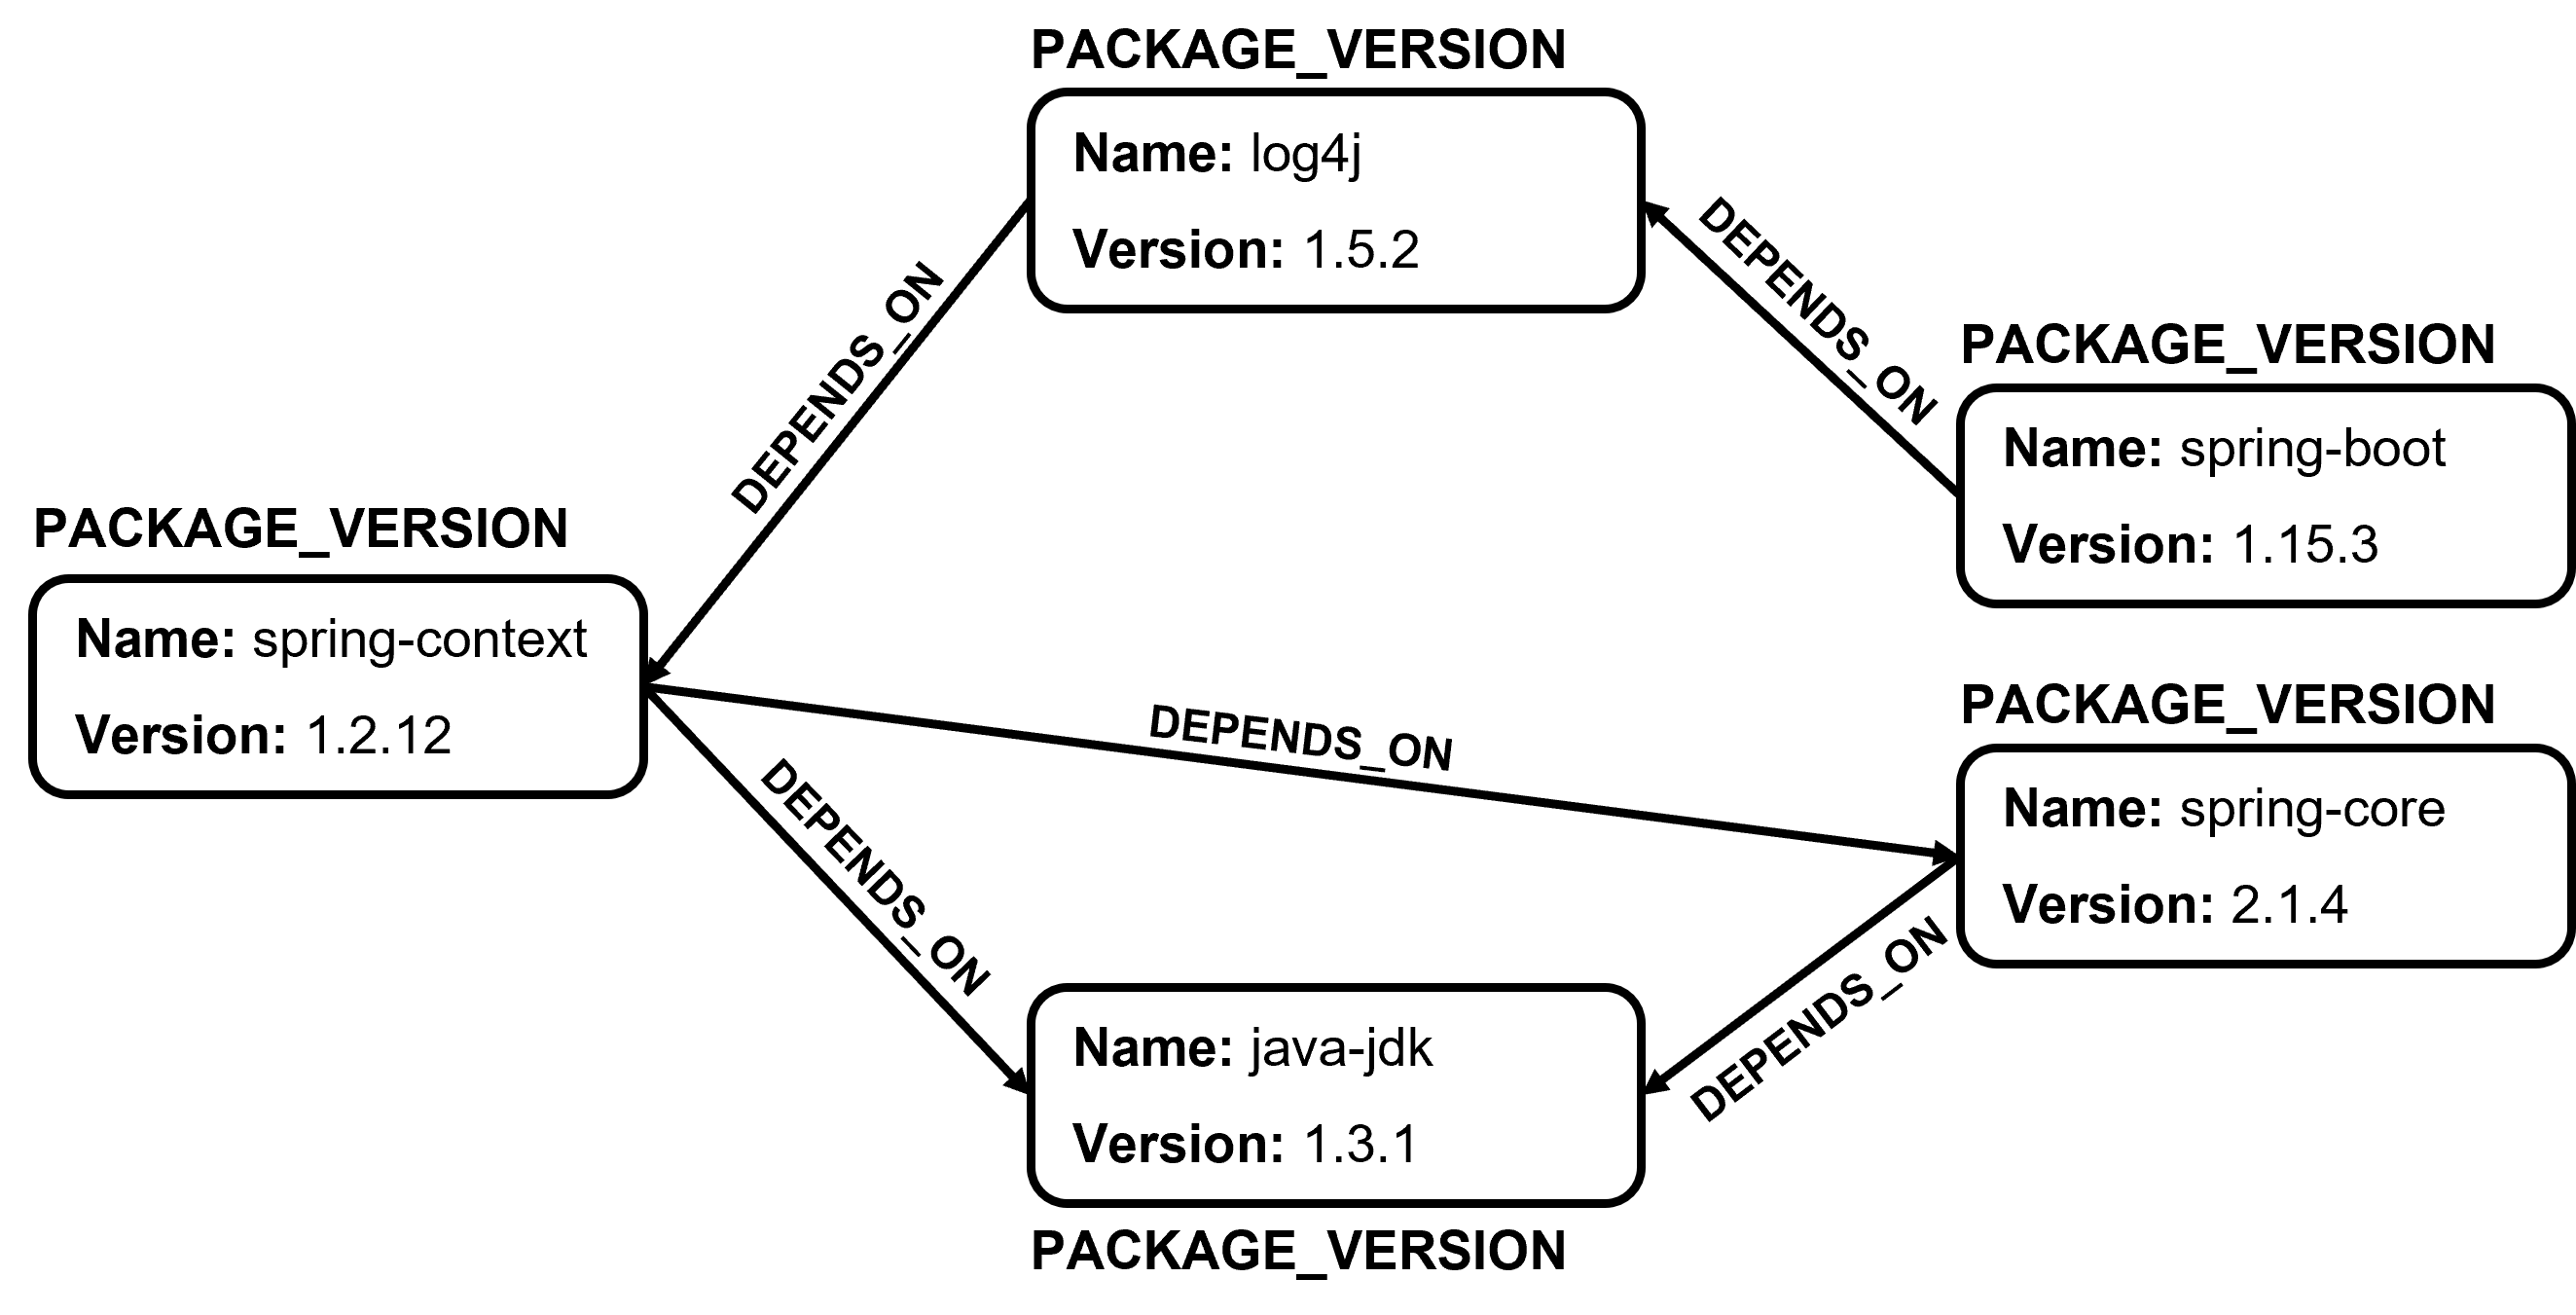
\includegraphics[scale=0.60]{dependency_graph}
	\caption[Package Versions and Dependencies as Graph]{Package Versions and Dependencies \source{Own Representation}}
	\label{fig:PackageVersionsAndDependenciesGraph}
\end{figure}

Neo4j defines its own SQL inspired language called \emph{cypher}. To answer the respective question ''Which Package Version does the spring-context:1.2.12 Package Version depend on?'' in Neo4j, the following cypher query would have to be used:

\begin{lstlisting}[caption=Package Version Dependencies (including transitive), captionpos=b, label=lst:CypherTransitive]
MATCH (p1:PACKAGE_VERSION {Name:''spring-context'',Version:''1.2.12''})
MATCH (p2:PACKAGE_VERSION)
WHERE (p1)-[:DEPENDS_ON*1..]->(p2)
RETURN (p2)
\end{lstlisting}

The first line in listing \ref{lst:CypherTransitive} matches the node with the \emph{label} \lstinline|PACKAGE_VERSION| and the key-value-pairs \lstinline|Name: ''spring-context''| and \lstinline|Version: ''1.2.12''| and assigns the resulting nodes, or in this example rather node as there is just a single one that fulfills this pattern, to the variable \lstinline|p1|. The second and third line match all nodes with the \emph{label} \lstinline|PACKAGE_VERSION| that \lstinline|p1| depends on. Thus, the \lstinline|WHERE| uses a path as a predicate. Thereby, \lstinline|DEPENDS_ON| specifies the \emph{label} of the relationship and the part after the asterisk specifies the minimum and maximum amounts of hops between the nodes. In this case, the minimum is 1 because with the default 0 it would consider itself and as there is no explicit maximum given, it defaults to infinite, to consider all transitive dependencies. The nodes that fulfill these criteria are assigned to \lstinline|p2| and returned, in this case, \emph{java-jdk 1.3.1} and \emph{spring-core 2.1.4}.\par 
Assuming there is a composite index on \emph{Name} and \emph{Version}, the initial look up of the node has a time complexity of $O(log(n))$ with $n$ being the number of all nodes with the label \emph{PACKAGE\_VERSION} \cite{neo4j}. The consecutive look ups then have a time complexity of $O(m)$ with $m$ being the number of nodes found during the previous look up. Thus, depending on the number of hops, the general time complexity for such a relationship traversal query may be estimated as 
$$O(log(n)) + O(m) + ... + O(m)$$

So theoretically, the graph database performs and scales significantly better than the relational database for this kind of queries. Besides, the query is definitely simpler to read and understand than the SQL query involving Common Table Expressions. Although, it is arguably still easier to learn the Common Table Expression than learning an entire new query language.\par 
Now just for completion, to answer the reciprocal question ''Which Package Versions depend on the spring-context:1.2.12 Package Version?'', the following cypher query would have to be used:

\begin{lstlisting}[caption=Package Version Reciprocal Dependencies (including transitive), captionpos=b, label=lst:CypherReciprocalTransitive]
MATCH (p1:PACKAGE_VERSION {Name:''spring-context'',Version:''1.2.12''})
MATCH (p2:PACKAGE_VERSION)
WHERE (p1)<-[:DEPENDS_ON*1..]-(p2)
RETURN (p2)
\end{lstlisting}

The only difference in this query is the reversed direction of the relationship in line 3. In this case, it return \emph{log4j 1.5.2} and \emph{spring-boot 1.15.3}. The respective cypher statements to set up the sample data are included in appendix \ref{apx:Data Definition Statement for Neo4J Sample Data}.\par
Besides the efficient traversal of relationship with rather simple queries, there are some other aspects to consider with graph databases. Generally, most graph databases support transactions with \emph{ACID compliance} \cite{neo4jtransactions, arangodbtransactions}. Also, there are some mechanisms to support \emph{referential integrity}, but those do not work exactly as in relational databases. So, in graph databases there is no way to create a relationship to or from a node that does not exist. Furthermore, nodes cannot be deleted as long as relationships to or from that node exist. But compared to relational databases, there is no option to cascade a delete \cite{neo4jdelete}.\par
Regarding \emph{schemas}, or the general storage model, different graph databases vary. Neo4j, for example, only supports key-value properties on nodes or relationships. This is considered as \emph{single model graph database}. In contrast, in ArangoDB every node is a JSON document, which is considered as \emph{multi model graph database} \cite{arangodbdocuments}. Therefore, Neo4j does not really have a classical schema. But it still offers several types of constraints such as \emph{unique node property constraints}, \emph{node property existence constraints} and \emph{relationship property existence constraints} to enforce a specific data model \cite{neo4jconstraints}. Similar to MongoDB, for ArangoDB a schema may be enforced on application level \cite{arangodbschema}.

\subsection{Database Selection}
In the following, a conclusion of this analysis of the suitability of database technologies for a central metadata store will be drawn.\par 
\emph{Relational databases} are a solid choice. As shown in the corresponding suitability section, modern SQL provides all features necessary to conveniently implement the required functionality. But the computational complexity of joins is 
$$O(log(n)) + O(m*log(n)) + ... + O(m*log(n))$$
As traversing relationships is involved in the prospectively most frequently used queries, this is a quite important measure.\par 
\emph{Document databases} are not the technology for this application. As it does not allow for significant de-normalization since the access patterns are versatile, the document database does not have an advantage over a relational database.\par 
\emph{Graph databases} are optimized for relationship traversal. The previous section has also shown that the cypher queries are simple in comparison to SQL. Due to its purpose, its computational complexity of traversing relationships is better than with relational databases
$$O(log(n)) + O(m) + ... + O(m)$$
So, the graph database seems to be the theoretically best database technology for this application. In practice, it also has to be considered that the application has to be supported and that there is less experience around graph databases in the industry. This also increases the chances of unforeseen queries or other situation, where the graph database may be a problem.\par 
\emph{For the scope of this work, the graph database is chosen for the implementation to further evaluate its suitability and practicality.}\\

The concrete graph database solutions considered were primarily Neo4j and ArangoDB. Neo4j because it has an open source community edition, good documentation and a supportive community. ArangoDB mainly because it is multi model and therefore enables storing JSON, which offers greater flexibility.\par 
Finally, Neo4j was chosen as it seemed to be the better fit over all. Even in the situations where JSON has to be stored, it is rarely necessary to traverse into the document structure. So it is usually sufficient to access the JSON document by its key which may also be done in Neo4j.

\section{Programming Language}
The \emph{programming language} used to implement the services comprising the Security and Compliance Data Lake is \emph{Go} \cite{Golang}. Generally, the services could probably be implemented with any common programming language. Therefore, the following application architecture design explanations and discussions are kept \emph{programming language-agnostic}.\par 
Since SAP Gardener is a managed Kubernetes service and Kubernetes is primarily written in Go, Go is the main programming language of the team. Therefore, Go was primarily chosen to fit in into the SAP Gardener ecosystem. This increases interoperability with other services of the team. But most importantly, this enables other members of the team to further maintain the application. 

\section{Application Architecture}
To further discuss the application and the other important design decisions involved, especially concerning the API, a rough understanding of how the application is composed may be helpful. Thus, the below figure \ref{fig:ApplicationArchitecture} illustrates the application's architecture. 

\begin{figure}[H]
	\centering
	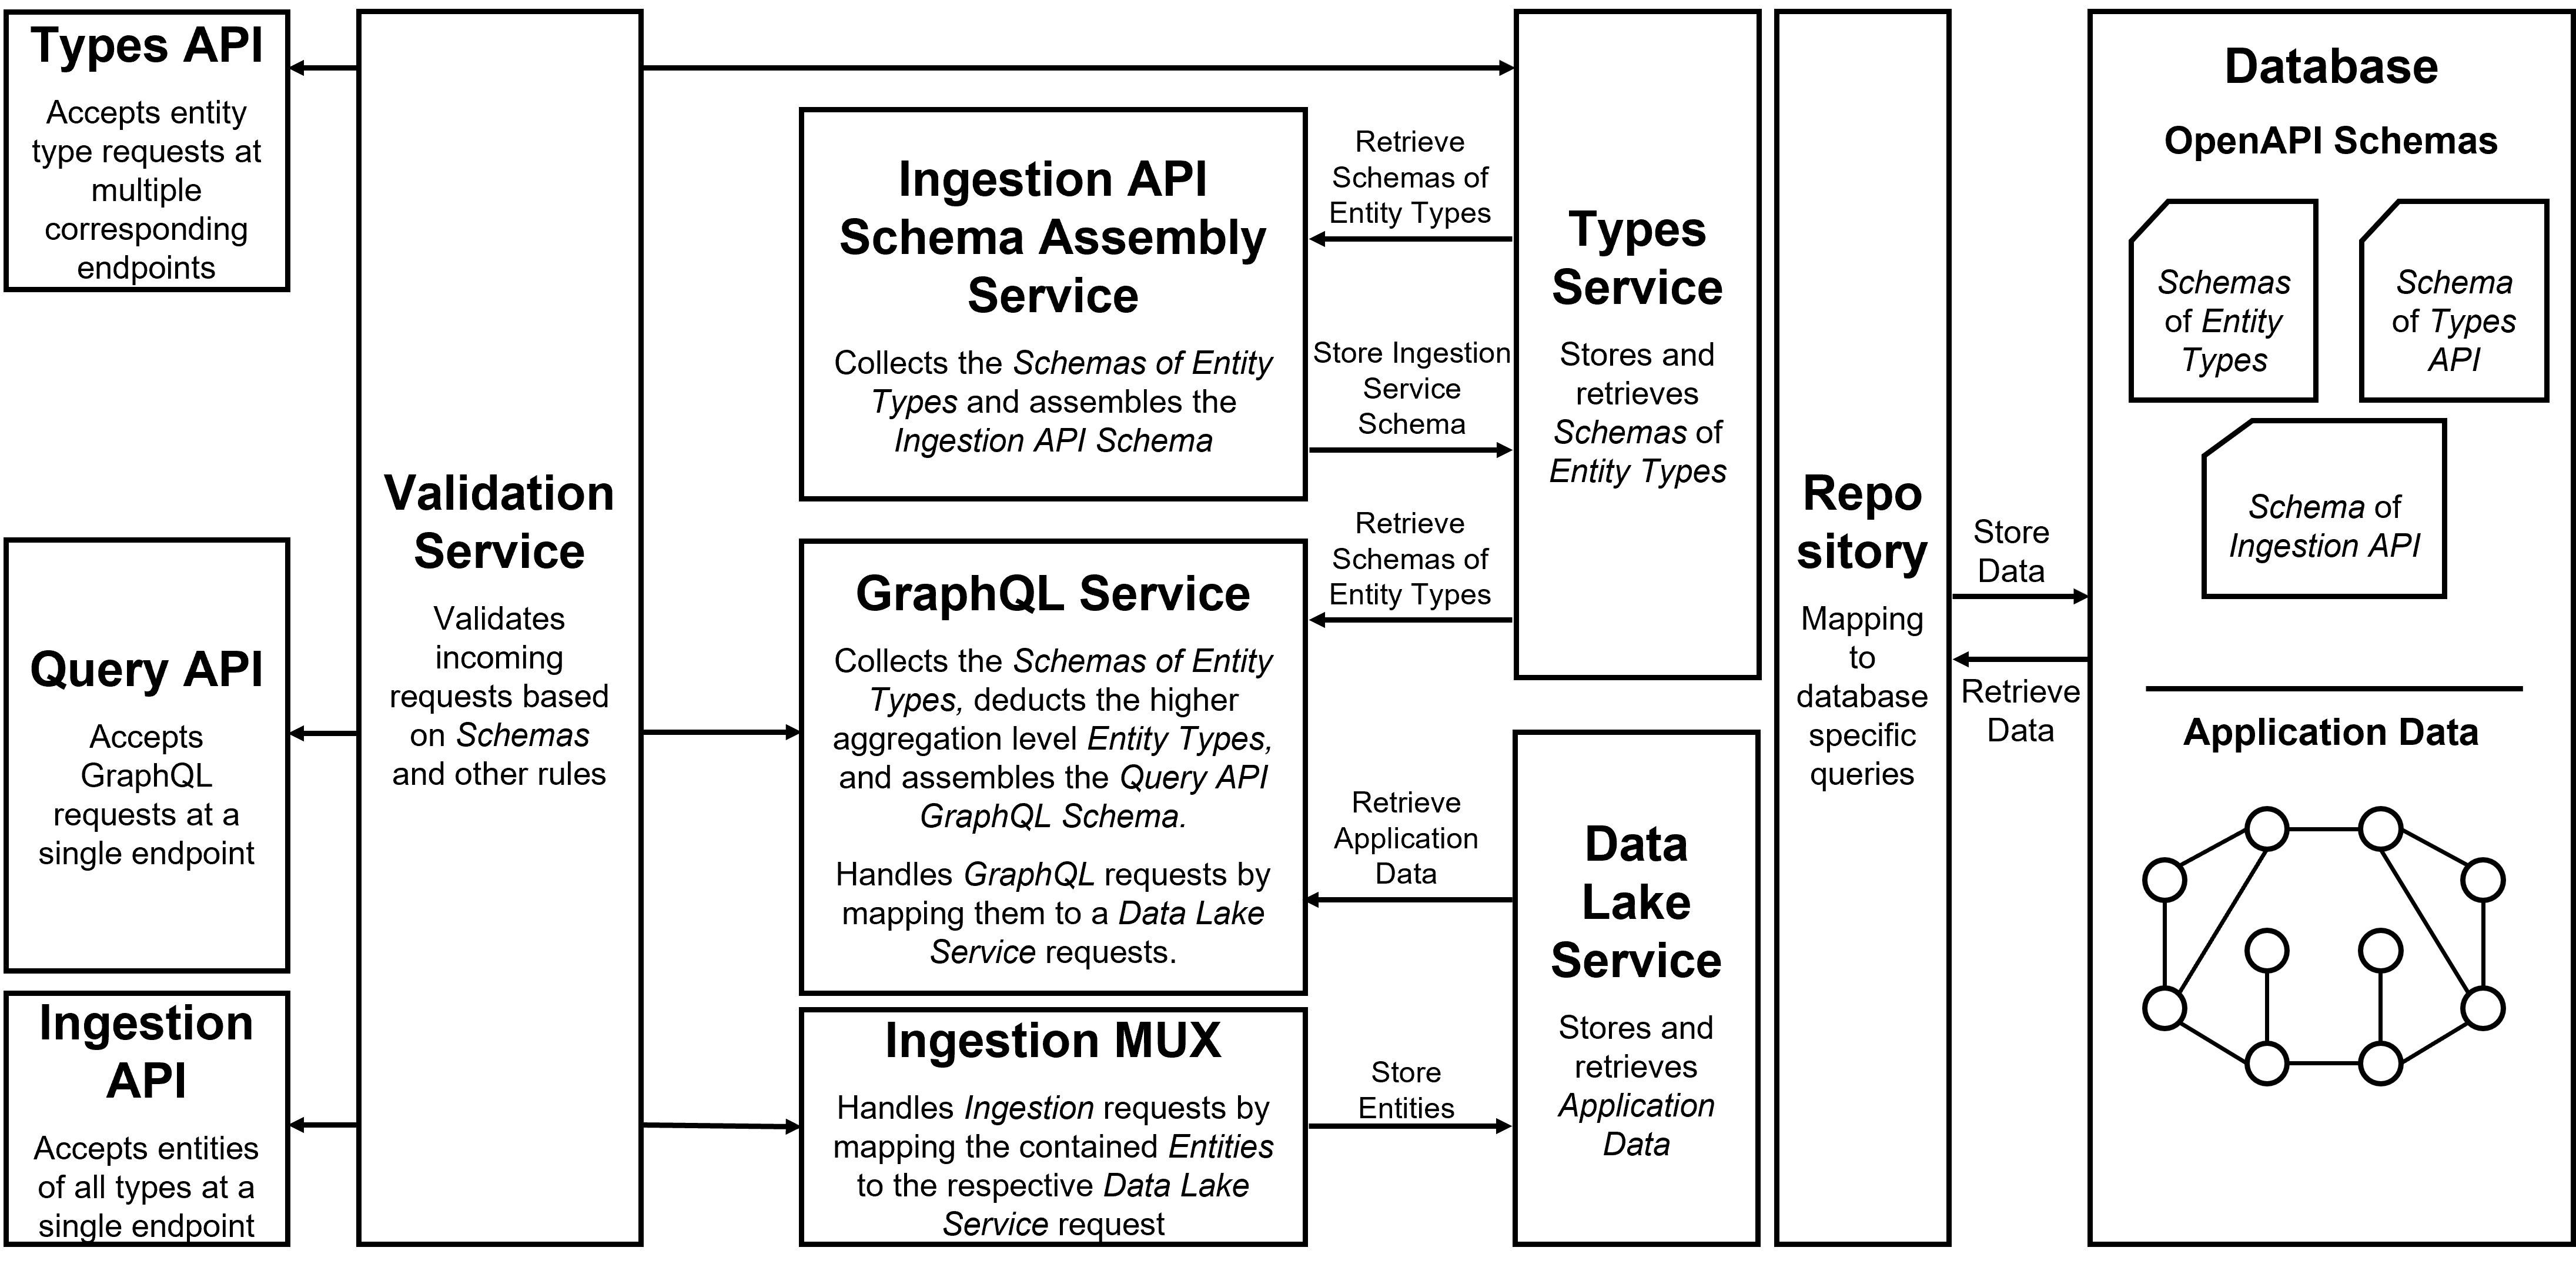
\includegraphics[scale=0.45]{application_architecture}
	\caption[Application Architecture]{Application Architecture \source{Own Representation}}
	\label{fig:ApplicationArchitecture}
\end{figure}

This section only provides an overview of the application. It thereby refers to standards and technologies, especially \emph{OpenAPI} and \emph{GraphQL}, that have not been properly introduced yet. This is done in the following \emph{API \& Services} sections along detailed explanations of the respective design decisions.\par
The application shall be independent of a specific component model and also open to a variety of data sources. To provide this flexibility and extensibility, the application's data model has to be configurable at runtime. This configurability, or in other words ability to instantiate the the meta data model as shown by the example in section \ref{sec:Application of the Data Model}, is offered through the \emph{Types API}, which allows the application administrator to define and adjust the data model to a specific use case. Therefore, \emph{OpenAPI} schemas of entity types have to be sent to an entity type specific endpoint of the \emph{Types API}. These OpenAPI schemas are then validated by the \emph{Validation Service}. Finally, the \emph{Types Service} stores the schemas in the database. Through this \emph{Types API}, the administrator is also able to retrieve existing schemas.\par
As shown in the figure, the \emph{Types Service} is the central service to store and retrieve schemas from the database. Correspondingly, the \emph{Data Lake Service} is the central service to store and retrieve application data. To make the application rather persistence agnostic, thus, to make it easy to exchange the underlying database, the services' interaction with the database is performed through an abstraction layer referred to as \emph{Repository}.\par 
To enforce the data model configured by the administrator, the \emph{Ingestion API Schema Assembly Service} retrieves the entity type schemas through the \emph{Types Service} and assembles them to a complete \emph{Ingestion API Schema}. This \emph{Ingestion API Schema} is then also stored in the database.\par
The entire \emph{Ingestion API} is based on this dynamically, at runtime, constructed schema. Thus, the \emph{Validation Service} validates every request with all entities to be stored against this schema, before it is passed on for further processing. The \emph{Ingestion API} exposes only a single endpoint instead of entity type specific endpoints. This makes the upload easier and more flexible from the adapter's perspective, as requests do not have to be routed to a specific endpoint. Furthermore, considering future performance optimizations, this allows sending larger chunks of data at once.\par
As the entities of different entity types still have to be processed differently, the \emph{Ingestion MUX} identifies the type of each entity contained in a request and routes it to the respective \emph{Data Lake Service} function.\par 
Finally, in order to being able to query the stored data based on the data model, the \emph{GraphQL Service} constructs a \emph{GraphQL} schema based on the \emph{OpenAPI} schemas of the entity types. The \emph{Query API} therefore also only exposes a single \emph{GraphQL} endpoint. The queries against this endpoint, thus, against the dynamically constructed \emph{GraphQL} schema, are resolved by corresponding functions of the \emph{Data Lake Service}.\\

The application architecture is essentially a \emph{layered architecture}. In the traditional sense of a the three principle layers, the \emph{APIs} represent the \emph{presentation logic layer} in above figure. Thus, the \emph{APIs} receive HTTP requests, interpret those requests into actions upon the \emph{domain layer} and return information to the user in form of a HTTP responses \cite{AppArchitecture}.\par
The \emph{Validation Service}, \emph{Types Service}, \emph{Ingestion API Schema Assembly Service}, \emph{GraphQL Service}, \emph{Ingestion MUX} and \emph{Data Lake Service} are on the \emph{domain logic layer}. Thus, these services validate data that comes in from the \emph{presentation layer} and perform tasks based on inputs and stored data \cite{AppArchitecture}.\par
Finally, the \emph{Repository} is on the \emph{data source logic layer} as it is responsible for communicating with the database to carry out tasks on behalf of the application \cite{AppArchitecture}.\par
Beyond that, these services are layered even further, as the services further left, thus, service on a higher layer, use functionality provided by services further right (relative to themselves), thus, services on a lower layer. But the lower layer services are unaware of the higher level services \cite{AppArchitecture}.

\subsection{Types API \& Services} \label{sec:Types API & Services}
As explained in the overview, every service of the application builds on the schemas which may be created through the \emph{Types API} and respective \emph{Services}. Thus, the rationale behind this service as well as the design decisions involved, are discussed first.\par

\subsubsection{Schema}
As the whole complexity of the architecture revolves around the dynamically configurable schemas, a common question especially considering the \emph{schema-less} database may be why the application even requires such rigid complete schemas?\par
The term \emph{schema-less} often leads to the misconception that the data somehow does not need to abide to any schema. Technically, this is true for most databases attributed with the term schema-less, like Neo4j. So the database will allow storing any key-value pairs. The problem is, without prior knowledge about the keys, the data cannot be retrieved. And without prior knowledge about the data types, the data may hardly be aggregated. Thus, even with schema-less databases, \emph{partial schemas} are enforced in most use cases.\par
In this context, partial schema usually means that the application requires a specific predefined set of properties with particular data types. But the application is not limited to those properties. Therefore, a set of unspecified properties may be stored alongside the data defined by a schema.\par 
Such partial schemas may be enforced by the database through constraints or by the application through frameworks, libraries and standards like \emph{JSON Schema} \cite{JsonSchema} and \emph{OpenAPI}.\\

The \emph{OpenAPI Specification (OAS)} is a technical specification defining a standard, programming language-agnostic interface description for HTTP APIs. The specification is maintained by the \emph{OpenAPI Initiative (OAI)} and is based on the \emph{Swagger Specification}, donated by \emph{SmartBear} who are also among the founding members \cite{OpenAPISpec}.\par
An OpenAPI document may be represented either in JSON or YAML format. To make this tangible, the below listing \ref{lst:SampleOpenAPI} shows a sample OpenAPI Document describing an exemplary HTTP API by leveraging the core concepts of the specification.

\begin{lstlisting}[basicstyle=\tiny, caption=Sample OpenAPI Document, captionpos=b, label=lst:SampleOpenAPI]
openapi: 3.0.0
  info:
    title: Sample API
    description: Serve as a Sample to explain OpenAPI
    version: 0.1.9
  servers:
    - url: http://api.example.com/v1
      description: Production Server
    - url: http://dev-api.example.com
      description: Development Server
	
paths:
  /customers:
    get:
      summary: Returns a list of customers.
      responses:
        200:
          description: A JSON array of users.
          content:
            application/json:
              schema:
                $ref: '#/components/schemas/Customers'
    put:
      summary: Merge a list of customers.
      requestBody:
        content:
          application/json:
            schema:
              $ref: '#/components/schemas/Customers'
        required: true
      responses:
        200:
          description: Customers merged successfully.
        400:
          description: Bad Request.
          content:
            application/json:
              schema:
                $ref: '#/components/schemas/Error'
  /customers/{id}:
    get:
      summary: Return a specific customer.
      parameters:
        - name: id
          in: path
          description: ID of a customer
          required: true
          schema:
            type: string
    ...
...
components:
  schemas:
    Customers:
      type: array
      items:
        $ref: '#/components/schemas/Customer'
    Customer:
      type: object
      required:
        - id
        - name
      properties:
        id:
          type: integer
        name:
          type: string
        address:
          type: object
          properties:
            city:
              type: string
            country:
              type: string
    Error:
      type: object
      properties:
        title:
          type: string
        status:
          type: string
        detail:
          type: string
\end{lstlisting}

The \emph{openapi} and the \emph{info} fields are both required. The \emph{openapi} field describes the version number of the OpenAPI Specification used. The \emph{info} field provides metadata about the API. The other fields are optional, although it is required that an OpenAPI document contains at least one \emph{paths}, \emph{components} or \emph{webhooks} field. As listing \ref{lst:SampleOpenAPI} has a \emph{paths} as well as a \emph{components} field, this requirement is fulfilled.\par
The paths describe the available endpoints of the API and their respective operations. Thus, \lstinline|/customers| and \lstinline|/customers/{id}| and the operations exposed through the HTTP verbs such as GET and PUT. Thereby, the formats of the \emph{content} in the \emph{requestBody} or in the \emph{responses} may be described, in this case \emph{application/json}. And most importantly, even a \emph{schema} may be provided for each respective content. Thus, the input and output data types may be specified. The specification, or rather schema, for these schemas is a superset of the JSON Schema Specification \cite{OpenAPISubset}.\par 
The \emph{components} field, or rather object, is a container for defining reusable objects which may be referenced. Most commonly, it is used to define reusable schemas as shown in listing \ref{lst:SampleOpenAPI} for \emph{Customers}, \emph{Customer} and also \emph{Error}. But it is also possible to specify entire \emph{responses}, \emph{requestBodies} and several other \emph{components} to make them reusable. If the \emph{component} is only used once, it may also just be defined in place, as shown for the schema of the \emph{id} parameter of the \lstinline|/customers/{id}| path's GET operation.\par
The schemas themselves are quite intuitive to read, write and understand. \emph{Customers} is an \emph{array} where each item is a \emph{Customer}. Meanwhile, \emph{Customer} is a \emph{object}, thus, an abstract data type, with two required properties, \emph{id} and \emph{name}, both of type \emph{string} and an optional property \emph{address} which itself is an object.\par
As shown by listing \ref{lst:SampleOpenAPI}, an OpenAPI document specifies an HTTP API in a format which allows both humans and computers to understand the capabilities of a service without requiring access to source code or additional documentation.\par
There is a ecosystem of tooling around OpenAPI documents. Most prominently, \emph{Swagger UI}, a tool which automatically generates a Web UI from OpenAPI documents for convenient visualization and interaction with the API \cite{SwaggerUI}. Furthermore, there are tools for server and client code generation, for request and response validation, for document serialization and deserialization and for testing in various programming languages \cite{OpenAPISubset}.\par
Several such tools are leveraged in the Security and Compliance Data Lake.\\

There is a rather simple reason, why this partial schemas approach to flexibility and extensibility is not sufficient for this application. The data, thus, the entities, are provided by other systems based on policies. Looking back at section \ref{sec:Reference Integration Architecture} ''Reference Integration Architecture'', the component model data may be fetched from a component repository once a day. Correspondingly, the artifact composition data, thus the packages contained in an artifact, may also be fetched from scanning tools once a day. To determine whether an entity such as a component or package already exists in the database, the application has to know the identity of the respective entity. But different component models may identify components by different sets of properties. Different scanning tools may identify packages by different sets of properties. Furthermore, different \emph{Info Snippets} such as vulnerabilities and license are unlikely to be identified by the same set of properties. Therefore, it is also impossible to predefine even a partial schema.\par 
The dynamically configurable schemas of this application are even implemented to be complete. So, the application does not really leverage the flexibility of using a schema-less database. This is because allowing properties that are not defined by a schema often leads to a decreased data quality as it entices to just store everything. Since properties not included in the schema are also rarely used in queries, they frequently do not add value.\par 
Besides, the real value provided by the application is the queryability of software composition. In the rare occasions where some information may be actually missing, it is easy to manually look it up in the original data source.  


\subsubsection{Meta Data Model} \label{sec:Meta Data Model}
Providing simple OpenAPI schemas would not be sufficient. A common OpenAPI component schema enables to define objects with a set of properties. Thereby, it may also be specified what data type these properties have and whether they are required \cite{OpenAPISpec}. While such a specification is enough for validation purposes, it lacks the information which properties are part of the entity type's identity.\par 
To solve this problem, the \emph{Types API} enforces a \emph{Meta Data Model}, which defines schemas for the entity type schemas. Below listing \ref{lst:EntityTypeSchemaSchema} shows the YAML representation of the \emph{Component Type} schema schema.

\begin{lstlisting}[basicstyle=\tiny, caption=Entity Type Schema Schema, captionpos=b, label=lst:EntityTypeSchemaSchema]
ComponentType:
  type: object
  required:
  - kind
  - version
  - name
  - identity_schema
  - attributes_schema
  properties:
    kind: 
      type: string
    version:
      type: string
    name:
      type: string
    identity_schema:
      type: object
    attributes_schema:
      type: object
\end{lstlisting}

Thus, the entity type schemas have to have a \emph{kind}, \emph{version}, \emph{name} and especially an \emph{identity\_schema} and an \emph{attributes\_schema} property. As the names suggest, the \emph{identity\_schema} and the \emph{attributes\_schema} of type object are themselves again schemas. The \emph{identity\_schema} thereby defines all the properties comprising the identity of the entity type and the \emph{attributes\_schema} specifies all other properties. As this is very abstract and meta level, below listing shows an exemplary JSON representation of a request body to create a \emph{Component Version} schema. 

\begin{lstlisting}[basicstyle=\tiny, caption=Request Body for Component Version Schema Creation, captionpos=b, label=lst:ComponentVersionSchemaCreation]
{
  ''kind'': ''ComponentType'',
  ''version'': ''v1alpha1'',
  ''name'': ''Component'',
  ''identity_schema'': {
    ''type'': ''object'',
    ''required'': [
      ''name'',
      ''version''
    ],
    ''properties'': {
      ''name'': {
        ''type'': ''string'',
        ''maxLength'': 255
      },
      ''version'': {
        ''type'': ''string''
      }
    }
  },
  ''attributes_schema'': {
    ''type'': ''object'',
    ''properties'': {
      ''labels'': {
        ''type'': ''array'',
        ''items'': {
          ''type'': ''object'',
          ''required'': [
            ''name'',
            ''value''
          ],
          ''properties'': {
            ''name'': {
              ''type'': ''string'',
            },
            ''value'': {}
          }
        }  
      }
    }
  }
}
\end{lstlisting}

So the identity of this \emph{Component Version} entity type is comprised of a \emph{name} property of type string and a maximum length of 255 characters and \emph{version} property also of type string with no further restriction. Both of these properties are required. The only further property in this example is \emph{labels}, which is an array of objects with a required \emph{name} property of type string and a \emph{value} property of any type. Thus, this array may hold arbitrarily nested objects.\par 
The other properties provided in this request, so \emph{kind}, \emph{version} and \emph{name}, are not part of the entity types schema. These properties are used for processing logic.\par 
\emph{kind} describes the \emph{class of entity types}.\par 
\emph{version} describes the version of the particular entity type schema. This property theoretically provides the possibility to update the entity type schema in case an additional property is required. But currently, the application does not provide any functionality to support such version upgrades by automatically updating the existing entities of that entity type.\par 
\emph{name} is the actual name of the entity type. Thereby, every node of that entity type will be labeled with this name (correspondingly, in a relational database, this would make up the name of the table). Thus, the \emph{name} is required when querying for nodes of that entity type in the database.\par
Based on the data model defined in the section \ref{sec:Data Model}, the combination of \emph{kind} and \emph{name} would only be necessary for \emph{Native Package Version} and \emph{Info Snippet} where multiple entity types of the same class of entity types, or rather \emph{kind}, may be created. In order to have uniform schemas but also especially for extensibility reasons, the application assumes all entity types in the data model may be classes of entity types. Therefore, the combination of the \emph{kind} and \emph{name} property is required to be included with all entity type schemas. This way, the application could be easily extended to store multiple component models.\\

Currently, these schemas cannot be provided for the abstract entity types, thus, \emph{Component}, \emph{Resource}, \emph{Source}, \emph{Package}, \emph{Package Version}, but only for their respective concrete entity types \emph{Component Version}, thus, \emph{Resource Version}, \emph{Source Version}, \emph{Native Package Version} and \emph{Info Snippets}.\par 
This is because these are the types of entities that are provided by the component model and data sources, thus, the types of entities that are actually ingested. Their abstract entities are rather groupings of those entities, thus, aggregations. As discussed in the data model section, these entities therefore mostly store information that has to be manually created by the user such as \emph{triage policies} or information that is merged from the concrete entities such as the common properties of \emph{Native Package Versions} in \emph{Package Versions}. Furthermore, especially the identities of the abstract entities depend on the respective concrete entity's identity.\par
For example, the identity of a \emph{Component} is equal to the identity of a \emph{Component Version} without considering the version property. Similarly for all other entities with a corresponding relationship. Therefore, although this unfortunately is not and cannot be represented in the OpenAPI schema of the entity types schema, the application enforces all the entity type's \emph{identity\_schemas} except the ones' of \emph{Info Snippets} to provide a \emph{version} property. While consuming and storing entities through the \emph{Ingestion API}, the higher aggregation level entities are then created implicitly with the respective identity.\par
The \emph{Ingestion API Schema Assembly Service} which builds the whole \emph{Ingestion API schema} retrieves the created schemas of the concrete  entity types and assembles \emph{identity\_schema} and \emph{attributes\_schema} to a single component schema for the entity type as shown in the listing below.

\begin{lstlisting}[basicstyle=\tiny, caption=Component Version Schema, captionpos=b, label=lst:ComponentVersionSchema]
''Component.v1alpha1'': {
  ''type'': ''object'',
  ''properties'': {
    ''metadata'': {
      ''type'': ''object'',
      ''required'': [''kind'', ''type'', ''version''],
      ''properties'': {
      	''kind'': {
      	  ''type'': ''string'',
      	  ''pattern'': ''^ComponentType$''
      	},
        ''type'': {
          ''type'': ''string'',
          ''pattern'': ''^Component$''
        },
        ''version'': {
          ''type'': ''string''
        }
      }
    },
    ''identity'': {
      ''type'': ''object'',
      ''required'': [''name'',''version''],
      ''properties'': {
        ''name'': {
          ''type'': ''string'',
          ''maxLength'': 255
        },
        ''version'': {
          ''type'': ''string''
        }
      }
    },
    ''attributes'': {
      ''type'': ''object'',
      ''properties'': {
        ''labels'': {
          ''type'': ''array'',
          ''items'': {
            ''type'': ''object'',
            ''required'': [''name'', ''value''],
            ''properties'': {
              ''name'': {
                ''type'': ''string'',
               },
              ''value'': {}
            }
          }  
        } 
      }
    }
  }
}
\end{lstlisting}

So, this is the schema against which entities of type \emph{Component Version} that shall be created through the \emph{Ingestion API} are validated. The \emph{metadata} properties are needed by the \emph{Ingestion MUX} in order to route the entity to the appropriate \emph{Data Lake Service} function.\\

This schema creation process is almost identical for all entity types, or rather classes of entity types, except for \emph{Native Package Version}. As common properties of different \emph{Native Package Version}, for example of BDBA and Mend, shall be merged on the \emph{Package Version} aggregation level, all \emph{Native Package Versions} have to share this set of common properties. Therefore, this creation process is slightly more modular, as will be shown in the next section discussing the endpoints.\par
Furthermore, there are currently predefined schemas for the \emph{Relationships} between the entity types. These schemas are all quite similar. They all require a \emph{source}, which refers to the identity of the entity type for which the relationship is outgoing, and a \emph{destination}, which refers to the identity of the entity type for which the relationship is incoming. Therefore, the schema for a \emph{Component Reference}, thus, for a \emph{Component Version to Component Version} relationship requires the identity of a \emph{Component Version} as a \emph{source} and as a \emph{destination}. Correspondingly, a schema for a \emph{Component Version to Resource Version} relationship requires the identity of a \emph{Component Version} as a \emph{source} and the identity of a \emph{Resource Version} as a destination. This is necessary in order to create the relationships independently of the entities which makes the creation process even more flexible.\par 
Imagine each \emph{Component Version} schema also includes references to all related \emph{Component Versions}. As entities, or rather nodes, have to exist before relationships including them may be created, this would require to resolve these dependencies and create a corresponding execution order. While the same may be done with the above approach, it also offers the possibility of creating all entities first and then all relationships. Of course, this comes at the cost of having to send the identities redundantly.\par 
Apart from that, all \emph{Relationship} schemas only have two further properties, the \emph{labels} property, which allows arbitrarily nested objects and a \emph{name} property of type string. As mentioned before, Neo4j can store JSON documents. But as each node and relationship only stores key-value pairs, nested properties are stored as string and cannot be leveraged in queries (except for using string comparisons, which is quite inefficient).

\subsubsection{Endpoints}
The \emph{Types API} exposes the following HTTP endpoints:

\begin{lstlisting}[basicstyle=\tiny, caption=Types API Endpoints, captionpos=b, label=lst:TypesEndpoints]
/types/component

/types/resource

/types/source

/types/info-snippets

/types/packages
/types/package-identity
/types/package-attributes
/types/package-native-attributes
\end{lstlisting}

Each endpoint accepts HTTP POST, PUT, GET and DELETE requests\footnote{The current version of the application at the time of writing the thesis actually just supports POST requests to those endpoints to create the schemas. But it is planned to extend this to also support GET request to retrieve the respective schemas and also PUT and DELETE requests to edit accidental mistakes in newly created schemas that are not used yet.} for managing one \emph{kind} of schemas, the \lstinline|/types/component| endpoint for \emph{Component Version} schemas, the \lstinline|/types/resource| endpoint for \emph{Resource Version} schemas, the \lstinline|/types/source| for \emph{Source Version} schemas, the \lstinline|/types/info-snippets| for \emph{Info Snippets} schemas and the other four endpoints for \emph{Native Package Version} schemas.\par
As indicated in the previous section, the creation process of the \emph{Native Package Version} schemas is similar to the \emph{Component Version} example, but more modular. Therefore, the \emph{identity\_schema} and the \emph{attributes\_schema} have to be created in separate requests to separate endpoints. Moreover, the \emph{attributes\_schema} is further broken down into \emph{attributes} and \emph{native attributes}, where \emph{attributes} is the set of properties that may be merged in the corresponding \emph{Package Version} entity. The individual schemas are then tied together by a request to the \lstinline|/types/packages| endpoint, referencing the respective \emph{identity}, \emph{attributes} and \emph{native attributes schemas}.\\

Finally, an open question may be, why even expose multiple endpoints? Especially considering that the \emph{kind} is present in the request anyway, as shown in listing \ref{lst:ComponentVersionSchemaCreation}. Thus, the further routing could also be handled by a custom multiplexer evaluating that property.\par
The primary reason that such a single endpoint approach is taken for the \emph{Ingestion API} but not for this \emph{Types API} is that they are used completely differently.\par
The \emph{Ingestion API} only has to \emph{consume} huge amounts of data that are provided by other systems. The \emph{Types API} is used by a human administrator to configure the application by \emph{creating}, \emph{reading} and in edge cases also \emph{updating} and \emph{deleting} schemas. Also, this is probably done only a few times during the entire application life time. Therefore, considering the entity type schemas as REST resources and exposing corresponding endpoints allows to benefit from the intuitiveness of a REST API leveraging the common HTTP verbs.\\

Besides, there is another inconvenience with APIs that expose only a single endpoint which enables to submit multiple different entity types in a single request.\par 
OpenAPI has a construct called ''oneOf'' which allows to specify that all entities and relationships in the request have to fulfill exactly \emph{one of} a specified set of schemas. Thus, generally OpenAPI supports specifying that kind of endpoint. The problem is, validation functions provided by OpenAPI libraries in any programming language cannot produce helpful error messages for that kind of endpoint when trying to validate the whole request.\par 
Imagine a request contains multiple entities. One of them is faulty. Now, the general validation function does not know what kind of entity this is supposed to be, thus, against which specific schema it has to be validated. It only knows that this faulty entity does not fulfill any of the provided schemas.\par
Therefore, in order to get helpful error messages, the validation would have to be implemented at a later point, evaluating the \emph{kind} property and calling the validation function individually for each entity in the request with the corresponding schema. But this is more of an implementation detail.

\subsection{Ingestion API \& Services}
The \emph{Ingestion API} is fairly simple, once the \emph{Types API \& Services} are understood. It exposes a single HTTP endpoint:

\begin{lstlisting}[caption=Ingestion API Endpoint, captionpos=b, label=lst:IngestionEndpoint]
/datalake
\end{lstlisting}

This endpoint only accepts HTTP PUT and DELETE requests\footnote{The current version of the application at the time of writing the thesis actually just support PUT requests. But as in production there will likely be cases where some entity or relationship has to be removed, it is planned to extend this to also support DELETE requests}. The operation performed by the application when receiving a PUT request is \emph{merging}, or in the SQL context rather known as \emph{upsert}, of the respective entities and relationships. The request is validated against the \emph{Ingestion API Schema} assembled by the \emph{Ingestion API Schema Assembly Service}.\par 
A REST API approach similar to the \emph{Types API} would not add much value here. The API has to consume huge amounts of data provided by other systems. Multiple endpoints would result in additional unnecessary requests. A single endpoint, on the other hand, makes the implementation of the adapters simpler and entities in a request may be bundled more flexibly.\par
The downside of such an endpoint, as previously mentioned, are having to deal with the obscure error messages or alternatively implementing a more complex validation. But this is more of an implementation detail and the effort to implement the more complex validation is comparably low considering the rest of the application.\par
Furthermore, such an API also requires additional efforts, as a custom multiplexer has to be implemented to handle the routing which is commonly done by libraries and frameworks based on the URL. Popular examples therefore are \emph{Java's Spring} \cite{Spring} or \emph{Javascript's Express} \cite{Express}. In the context of the \emph{Ingestion API}, this routing is handled by the \emph{Ingestion MUX} individually for each entity in the request based on its \emph{kind} property. 

\subsection{Query API \& Services} \label{sec:Query API & Services}
While the \emph{Types API} and \emph{Ingestion API} may be interesting to administrators and adapter developers, the \emph{Query API} is the part of the application which actually provides value. Therefore, the \emph{Query API} and respective \emph{Services} have to enable users to conveniently perform queries and analysis by traversing relationships to answer questions such as ''Which Component Versions contain the Log4J Vulnerability?''.\par
A brief summary of the API development process may help in understanding the design decisions that led to the current \emph{GraphQL API}. 

\subsubsection{REST API}
REST APIs are currently probably the most popular types of APIs. This is due to their simplicity and intuitiveness leveraging the built in semantics of the web, the HTTP verbs, and mapping the main entity types of an application to resources and exposing them through individual endpoints.\par
Therefore, the initial idea was to design a single REST API for \emph{querying} as well as \emph{consuming} the data. Thus, at that point a separation of \emph{Ingestion API} and \emph{Query API} was not planned yet.\par 
There were several different approaches for endpoint design. There was the common mapping of entity types and relationships to resources and corresponding endpoints. And there were several different deviations of the common REST approach, trying to deal with the same \emph{three main problems} the classic REST API is facing in this use case.\par 
The below listings outlines the endpoints of a common mapping of the entity types and relationships to resources for the example of the component entity types:

\begin{lstlisting}[basicstyle=\tiny, caption=REST API Endpoints, captionpos=b, label=lst:RESTAPIEndpoints]
/components
/components/{component_name}
/components/{component_name}/versions
/components/{component_name}/versions/{version}
/components/{component_name}/versions/{version}/component_version_references
/components/{component_name}/versions/{version}/source_version_references
/components/{component_name}/versions/{version}/resource_version_references
\end{lstlisting}

There is a problem arising from such common REST API design regarding the \emph{data ingestion}. Theoretically, to create \emph{Component Versions}, the adapter would have to send a \emph{huge number of separate requests} and route them to the correct endpoints. Thus, to merge a version v0.15.0 of the component named \emph{github.com/gardener/etcd-druid}, a PUT request would have to be sent to \lstinline|/components/github.com/gardener/| \lstinline|etcd-druid/|. To merge the relationships, further PUT requests would have to be sent to the respective endpoints. This would result in a lot of separate requests. The relationships could not be created before the \emph{Component Version} exists. Thus, even the sequence of the requests is important. Therefore, this approach is impractical.\par
But, considering that the data sources only provide the lowest aggregation level entities, thus, \emph{Component Versions}, and the respective higher aggregation level entities, thus, \emph{Components}, usually are created implicitly anyway, a deviation from the REST standard for data ingestion was deemed acceptable. Therefore, to solve this problem, all \emph{Component Version} entities could just be sent to the \lstinline|/components| endpoint with the references as nested objects.\\

There is another problem concerning the \emph{queryability} of this REST API. Designing endpoints like this does enable to retrieve all information about the individual entities, but it does not provide a possibility to traverse the relationships with a single request. As the relationship itself is not really interesting for most queries, this problem could be solved by adding following endpoints:

\begin{lstlisting}[basicstyle=\tiny, caption=REST API Query Endpoints, captionpos=b, label=lst:RESTAPIQueryEndpoints]
/components/{component_name}/versions/{version}/component_versions
/components/{component_name}/versions/{version}/source_versions
/components/{component_name}/versions/{version}/resource_versions
/components/{component_name}/versions/{version}/package_versions
/components/{component_name}/versions/{version}/vulnerabilities
/components/{component_name}/versions/{version}/licenses
...
/components/{component_name}/components
/components/{component_name}/sources
/components/{component_name}/resources
/components/{component_name}/packages
/components/{component_name}/vulnerabilities
/components/{component_name}/licenses
...
\end{lstlisting}

So, the REST API would also enable to traverse the graph and intuitively answer the most common questions. Through URL parameters, further filtering of the corresponding result set would also be possible.\\

This deviation of a REST API seemed simple and intuitive and still powerful. But there is a third problem, \emph{parsing}. In the end, this also led to the final reason for not pursuing this approach further.\par
Part of the problem is already visible in the data ingestion example. Common routing frameworks and libraries are not able to handle URLs such as \lstinline|/components/| \lstinline|github.com/gardener/etcd-druid/| since the slashes in the name would be interpreted as a path separator.\par 
Intuitively, this could be solved by replacing the slash by a different character such as an underscore. But for this to work properly, the respective character cannot be allowed to be used in the name. This would definitely cause compatibility issues with OCM and other component models.\par 
Another approach is to implement a custom parser. But in order for this to work, the URLs have to be adjusted to always end on a keyword. For example, the previous URL to retrieve a component with a specific name would have to be changed to something like \lstinline|/components/github.com/| \lstinline|gardener/etcd-druid/list| with \emph{list} being the keyword. Then a custom parser could parse the URL backwards.\par
But even with URLs always ending on keywords, the parsing may not be unambiguous, as shown by the listing below.

\begin{lstlisting}[caption=Ambiguous REST API URL, captionpos=b, label=lst:Ambiguous URL]
/components/github.com/gardener/etcd-druid/versions/1.2.3/list
\end{lstlisting}

This request could be meant to list all \emph{Component Versions} with \emph{component\_name = github.com/gardener/etcd-druid}. But it could also be meant to list all \emph{Components} with \emph{component\_name = github.com/gardener/etcd-druid/versions/1.2.3}.\par
The problems become even more difficult to deal with when considering corresponding endpoints for \emph{Sources} and \emph{Resources}. Using the identity properties of the OCM, respective endpoints would look like this:

\begin{lstlisting}[caption=REST API Source Endpoint, captionpos=b, label=lst:RESTAPISourceEndpoint]
/sources/{component_name:component_version:source_name:extra_id}
\end{lstlisting}

While this is not really clean, it still seems as this may work as long as the character separating the individual properties of the sources' identity, in this example the colon, is guaranteed to not occur within one of the properties. But as previously established, such a separator would lead to compatibility issues. Besides, per OCM specification, the \emph{extra\_id} is a flat map containing an arbitrary number of key-value pairs. Thus, the key-value pairs would have to be included in the URL.\par
Therefore, it is apparent that there is no clean solution to identifying entities by integrating their dynamically configurable identities into the URL.\\

To solve this parsing issues, assigning additional \emph{surrogate keys}, thus \emph{UUIDs} or \emph{auto incremented IDs}, as it is done in common REST API use cases was considered. But this would require additional requests to find the surrogate key of the respective entity. Thus, the API would have to support requests using query parameters as indicated by the listing below.

\begin{lstlisting}[caption=Querying for Entitiy ID, captionpos=b, label=lst:QueryingForEntityID]
/sources?component_name=github.com/gardener/etcd-druid&version=0.15.0&source_name=etcd&extra_identifier=etcd-druid-source

/sources/{id}/versions
\end{lstlisting}

The user would first send the first request to retrieve the ID of the respective \emph{Source}. Once the ID is acquired, it might be used to navigate further through the API and, for example, retrieve all versions of the \emph{Source} with that ID.\par
Although every API that exposes its operations through individual resource endpoints is called REST API today \cite{RichardsonMaturityModel}, this form of usage is already much closer to the original REST architectural style defined by Roy Fielding. It is derived from the web and promotes hypermedia as the engine of application's state \cite{RESTArchitecturalStyle}. Thus, the original idea is that RESTful architectures and consequently also REST APIs may be navigated just as websites. So a user may know the host address of the API. Sending a GET request to that host address will then return a list of hyperlinks of further resources. For this API this may be \lstinline|/components|, \lstinline|/sources|, ... . Again, following one of those hyperlinks by sending a GET request will return another list of hyperlinks of further resources available under the currently selected resource, in the case of \lstinline|/components| a list of hyperlinks to all available individual \emph{Components}. This is great for APIs that have a potentially huge number of unknown users, as it is very intuitive and requires almost no documentation to navigate through, just as a website. But it is not suitable and creates a lot of overhead for this kind of application which requires running specific potentially expensive queries based on already known entities.\\

Finally, hashing the identity properties and using the hash as ID was considered. While this would allow to issue the queries directly without having to retrieve the ID first, it would require to calculate the hash. Due to implications regarding normalization, this would require an additional small program in order to being able to use the API. Therefore, this approach also was not pursued further.

\subsubsection{Remote Procedure Calls}
As the REST API approach was deemed unsuitable after thorough analysis, the next best idea was to implement the most common queries as \emph{Remote Procedure Calls (RPC)}.\par 
This approach is simple and clean. The application specifies a set of functions, or rather procedures, that may be called through the API. Furthermore, it defines which properties have to be provided for each procedure and the format in which these properties have to be provided. In the context of web services, those procedures are typically called by HTTP POST requests, specifying the procedure to be called as well as the corresponding properties in the corresponding format in the request body. Thus, there would be no issues regarding embedding properties in the URL and parsing.\par
While implementing the most common queries is convenient, it is also quite inflexible. An intuitive, more flexible approach which gives users the full capability to run precise and complex queries through the API and to answer questions such as ''Which Package Versions depend on the spring-context:1.2.12 Package Version?'' is indicated by the listing below.

\begin{lstlisting}[caption=Exposing Cypher through API, captionpos=b, label=lst:CypherThroughAPI]
POST /processCypher(
 ''MATCH (p1:PACKAGE_VERSION {Name:''spring-context'',Version:''1.2.12''})
  MATCH (p2:PACKAGE_VERSION)
  WHERE (p1)<-[:DEPENDS_ON*1..]-(p2)
  RETURN (p2)''
)
\end{lstlisting}

Thus, exposing the entire database query language through the API. But compared to the REST API, where answering such a question did not require any knowledge about graph databases, for this approach, the user has to know the entire database specific query language. And even then, the queries may be quite error prone. Besides, there are several security implications which make this approach impractical.\par
The basic idea of exposing a query language through the API is still powerful. But the set of available operation has to be smaller and the permissions stricter than the ones' of the database's query language. Thus, in the past there were a few attempts to design such API query languages - for example SPARQL, FIQL and a lesser-known one by Meta, FQL \cite{APIYouWontHate}. While these API query languages may be unsuitable for graph traversal, designing a language tailored to this application would be an option. But this would be quite time intensive and complex. Besides, the general problems with such API query languages are similar to exposing the database query language. Users have to be skilled in those languages in order to being able to use the API properly.\par
Thus, these RPC approaches were not satisfying either.

\subsubsection{GraphQL}
On a basic level, a \emph{GraphQL API} is also essentially RPC, as \emph{GraphQL} is also a query language for APIs \cite{GraphQL} designed by Meta. Thereby, a GraphQL API exposes a single endpoint which is typically called \lstinline|/graphql|.\par
But GraphQL has a special approach to specifying APIs and defining queries, which makes it very intuitive and easy to use. A GraphQL API is defined by \emph{types} which correspond to resources in a REST API, and \emph{fields} on this \emph{types}. To specify those \emph{types} and \emph{fields}, GraphQL provides its own \emph{GraphQL schema language}. Listing \ref{lst:GraphQLComponentVersion} shows an exemplary GraphQL schema language representation of a \emph{Component Version} based on the OCM data model instance in section \ref{sec:Application of the Data Model} ''Application of the Data Model''.

\begin{lstlisting}[basicstyle=\tiny, caption=GraphQL Component Version Schema, captionpos=b, label=lst:GraphQLComponentVersion]
type Query {
  Component(Identity: ComponentIdentityArgs): [Component]
  ComponentVersion(Identity: ComponentVersionIdentityArgs, Attributes: ComponentVersionAttributesArgs): [ComponentVersion]
  ...
}
type ComponentVersion {
  Identity: ComponentVersionIdentity
  Attributes: ComponentVersionAttributes
  IncomingReferences(type: String, name: String, labels: String): [Reference]
  OutgoingReferences(type: String, name: String, labels: String): [Reference]
  ReferencedComponents(Identity: ComponentIdentityArgs): [Component]
  ReferencedComponentVersions(Identity: ComponentVersionIdentityArgs, Attributes: ComponentVersionAttributesArgs): [ComponentVersion]
  ReferencedResources(Identity: ResourceIdentityArgs): [Resource]
  ReferencedResourceVersions(Identity: ResourceVersionIdentityArgs, Attributes: ResourceVersionAttributesArgs): [ResourceVersion]
  ReferencedSources(Identity: SourceIdentityArgs): [Source]
  ReferencedSourceVersions(Identity: SourceVersionIdentityArgs, Attributes: SourceVersionAttributesArgs): [SourceVersions]
  ContainedPackages(Identity: PackageIdentityArgs, Attributes: PackageAttributesArgs): [Package]
  ContainedPackageVersions(Identity: PackageVersionIdentityArgs, Attributes: PackageVersionAttributesArgs): [PackageVersion]
  ContainedBDBAPackageVersions(Identity: BDBAIdentityArgs, Attributes: BDBAAttributesArgs): [BDBAPackageVersion]
  ContainedVulnerabilities(Identity: VulnerabilityIdentityArgs, Attributes: VulnerabilityAttributesArgs): [Vulnerability]
}
type ComponentVersionIdentity {
  name: String
  version: String
}
type ComponentVersionAttributes {
  labels: String
}
...

input ComponentVersionIdentityArgs {
  name: String
  version: String
}
input ComponentVersionAttributesArgs {
  labels: String
}
...
\end{lstlisting}

The GraphQL schema language is quite intuitive. The \emph{Query} \emph{type} is a special type which defines the entry point for GraphQL queries, listing all \emph{types} a user may query for. These available \emph{types} further specify their fields and therefore declare what may be queried on them, and so on. Thereby, the GraphQL schema resembles a REST API which properly implements hypermedia as the engine of application state. But instead of having to send multiple queries to navigate through the API step by step and actually retrieve data, with GraphQL the entire schema may be retrieved at once. This reduces the overhead in requests and data transfer significantly.\par
The \emph{Component Version} \emph{object type} is a field within the \emph{Query} \emph{type} and has two \emph{ input objects} as arguments, the \emph{ComponentVersionIdentityArgs} object and the \emph{ComponentVersionAttributesArgs} object, defined at the bottom of the listing. \emph{[ComponentVersion]} thereby represents an array of \emph{Component Version} objects.\par 
The basic structure of the previously described REST API and of the GraphQL API defined by this schema is quite similar. Both hide the relationship traversals necessary to answer questions such as ''Which Vulnerabilities are contained in Component Version ''github.com/gardener/etcd-druid:0.15.0''?''. Instead, for the user of the API, it looks and feels like \emph{Component Versions} are stored like documents in a document database with all related entities directly nested inside of them. Thus, a GraphQL query to answer the respective question based on the above GraphQL schema looks like this:

\begin{lstlisting}[basicstyle=\tiny,  caption=GraphQL Query, captionpos=b, label=lst:GraphQLQuery]
{
  ComponentVersion(Identity: {name:''github.com/gardener/etcd-druid'', version: ''0.15.0''}) {
    ContainedVulnerabilities {
      Identity {
        cve
      }
      Attributes {
        summary
        cvss 
      }
    }
  }
}
\end{lstlisting}

In reality, the application assigns functions to the respective fields on a GraphQL schema. These functions generate a corresponding \emph{cypher} query to retrieve the data from the database and resolve the request.\par
As shown in listing \ref{lst:GraphQLQuery}, the query language even allows to specify which properties of the \emph{Vulnerabilities} shall be retrieved. While this is not really significant for this application, compared to a REST API this may reduce the overhead even further by exactly describing what shall be queried and retrieved.\par 
More importantly, the GraphQL query language gets rid of parsing issues as the data model and queries do not have to be mapped to URL paths. Additionally, it is also more powerful than the REST API, as it supports arbitrary nesting of the queried objects. Thus, considering above query, it is possible to specify to retrieve all packages the respective \emph{Vulnerability} occurs in. Depending on the exact GraphQL schema of the \emph{PackageVersion} \emph{type} the respective query would look something like this:

\begin{lstlisting}[basicstyle=\tiny, caption=Nested GraphQL Query, captionpos=b, label=lst:NestedGraphQLQuery]
{
  ComponentVersion(Identity: {name:''github.com/gardener/etcd-druid'', version: ''0.15.0''}) {
    ContainedVulnerabilities {
      Identity {
        cve
      }
      Attributes {
        summary
        cvss 
      }
      PackageVersions{
        Attributes {
          name
        }
      }
    }
  }
}
\end{lstlisting}

Thus, as GraphQL provides a clean, intuitive and powerful API, this is the approach that was finally selected for the Query API. GraphQL also has capabilities to manipulate data, but for this application, these are also less suitable than the \emph{Ingestion API}.\par
As already mentioned, the application cannot define the GraphQL schema statically. Instead, the schema has to be created and adjusted dynamically by the application based on the OpenAPI schemas created through the \emph{TypesAPI}. This is the biggest downside of this approach, as this is cumbersome to implement and adds a lot of complexity to the application.

\subsection{Limitations and Problems} \label{sec:Limitations and Problems}
The current application design as presented in the previous sections is not flawless and has limitations.\par 
The main limitation of the current design is the \emph{lack of explicit schemas for higher aggregation level entity types} and the \emph{implicit creation of the respective entities}. Generally, this is rather convenient for administrators, adapter developers as well as users of the API, as the ability to query the software composition on multiple aggregation levels comes seemingly for free. The administrator does not have to configure respective schemas for \emph{Component}, \emph{Source}, \emph{Resource}, \emph{Package}, \emph{Package Version} and \emph{Relationships}. Instead, only the schemas of entity types he is actually dealing with have to be configured, as the respective entities are provided by the component model and other data sources. And the adapter developer does not have to deduct these entities and send them to the API as their creation is handled implicitly by the application itself. So, for most use cases, this \emph{hides complexity} and may even be seen as an \emph{advantage}.\par
But answering questions about the software composition is not the sole purpose of the application. Looking back the requirements in sections \ref{sec:Requirements}, the application shall also enable assessments (R.6). The data model section \ref{sec:Data Model} therefore mentioned that \emph{triage policies} may be defined on \emph{Sources} and \emph{Resources} and the actual \emph{triage} information shall be stored on the relationships such as between \emph{Component Versions} and \emph{Source Versions} or \emph{Resource Versions}. Furthermore, these higher aggregate level entities shall be able to store semantic information about the grouping. These capabilities are not enabled by the current application design.\par
There are essentially two approaches to adjusting the application to support this functionality. One approach would be to explicitly deduct the \emph{identity\_schemas} for higher level entity types such as \emph{Component}, thus, the \emph{Component Versions} \emph{identity\_schema} without the \emph{version} property, and expose additional \emph{Types API} endpoints to add \emph{attribute\_schemas}. Possibly, to provide even more flexibility, the \emph{identity\_schema} of the higher level entity types could even be configured themselves as any subset of the lower level entity type instead of being predefined as the set of the lower entity types indentity properties excluding \emph{version}. Correspondingly, \emph{Types API} endpoints may be added to define the schemas of \emph{Relationships}. This approach matches the general extensibility and flexibility of the application, but also requires the most efforts to implement and adds a substantial amount of complexity for the administrators.\par
The other option is to statically predefine the properties available for \emph{triage policies} and \emph{triaging}. To add general semantic information, a \emph{labels} property which may store arbitrary key-value pairs may be added. This approach is quite low effort and does not add any complexity, but it is significantly more rigid. Also, the \emph{labels} property does not enable proper filtering upon the nested properties.\par
As the \emph{Ingestion API} is tailored towards handling huge amounts of data provided by other systems, an additional \emph{Triage API} may be added to manually store this information.\\

Furthermore, the flexibility and extensibility of the application comes at the cost of \emph{complexity}. This is partially represented in the previous sections, especially the \emph{Types API \& Services} with its \emph{Meta Data Model}. But it is also especially represented in the application's code. The code dealing with schema creation and translation, thus, the code making up the \emph{Ingestion API Schema Assembly Service} and \emph{GraphQL Service}, is quite lengthy. As the data types are not predefined, the whole application code has to work extensively with abstract data types such as maps\footnote{The name of this abstract data type varies between programming languages. Other common terms are associative array or dictionary.}, while leveraging reflection and casting. Furthermore, the whole processing logic had to be designed to being able to handle this level of flexibility. Even data base queries are constructed dynamically based on the respective configured schemas. This makes \emph{application maintenance} more difficult and error prone. Moreover, the implications of this amount of flexibility and extensibility for the \emph{application's security}, especially also concerning attacks like ''SQL injection'', have not been sufficiently analyzed and estimated so far. 